\documentclass[../primer.tex]{subfiles}

\begin{document}

\chapter{Formulate} \label{ch:formulate}
%% --------------------------------------------------
Any engineer or scientist worth their salt approaches a new problem first by
\textbf{formulating} it. This involves posing the the question(s) to be
answered, gathering relevant data and information, and obtaining or building
relevant models. Often we will need to post-process these models with some form
of sensitivity analysis, in order to support other UQ efforts. This chapter
focuses on tools and concepts to aid in the formulation stage, with a particular
eye towards handling uncertainty.

We start with the most important step: What \emph{question} or \emph{questions}
are we attempting to answer? This critical component will inform all following
work, and so should be posed as early as possible.

%% --------------------------------------------------
\section{Questions} \label{sec:questions}
%% --------------------------------------------------
``First secret: The most important question is the question.'' -- Andrea
Saltelli\cite{saltelli2000sensitivity}

The most important element of this process is unfortunately the most difficult
for us to provide specific advice; `the question' depends on the context, and is
inherently a value judgement on the part of the investigator. However, the
top-level inquiries in engineering and scientific applications often lead to
similar sub-questions, of which we can provide some examples.

An engineer may ask ``How can I design a safe, cost-effective bridge to cross
this river?'' This naturally leads to the question ``How can I measure safety of
a given design?'', which is commonly posed as a probabilistic (reliability)
problem. The engineer should also ask ``What models will be appropriate for this
design task?'' This may lead the engineer to seek a validated structural
analysis simulation code to aid in design. An engineer should also ask ``What
are my constraints and requirements for design?'' Some of these factors in
design may be uncertain, such as wind loading conditions.

A scientist may ask ``How can I better understand the interaction between fluid
and particles in a turbulent flow?'' The scientist should ask ``what observable
characteristic of the flow will enable me to understand particle-fluid
interactions?'' Often, the turbulent kinetic energy (TKE) is used to
characterize turbulent flows, so one might measure changes in TKE due to the
addition of particles. A scientist should always ask ``what is already known
about this phenomenon, and what is \emph{not} known?'' which may be answered by
literature review and conversations with peers.

Once the high-level objective of an investigation has been established, the
analyst should ask a number of follow-up questions:

``What do I need to know?'' What knowledge is necessary to build an appropriate
model for the problem, and what data is necessary to feed the model? What
assumptions will be appropriate for the problem at hand? Gathering this
information is necessary for further analysis -- failure to pose appropriate
assumptions or obtain relevant data can seriously cripple further efforts.

``Do I trust my data?'' When studying data, one should exercise some amount of
skepticism, especially when approaching a new dataset. Errors can enter data
very easily -- easy sanity checks can help to catch such problems. One should
also question whether the data are representative of the problem to be studied.
Section \ref{sec:data} provides some tools and concepts to study data and
exercise skepticism towards a dataset.

``Do I trust my assumptions?'' If the data are \emph{truly} representative of
the problem to be studied, then one can test assumptions against the data. Note
that this is a one-way diagnostic -- one can only falsify an assumption, not
`prove' that assumptions are true! Assuming that one can operationalize an
assumption as a model, Section \ref{sec:models} introduces some concepts to
question and quantify the validity of assumptions. Section \ref{sec:sa} provides
some tools to help investigate models, Section \ref{sec:inverse-propagation} of
Chapter \ref{ch:wrangle} gives examples of model sanity checks using inverse
propagation, and Chapter \ref{ch:act} gives examples of validation in practice.

%% --------------------------------------------------
\section{Uncertainty} \label{sec:uncertainty}
%% --------------------------------------------------
\textbf{Uncertainty} is the primary subject of this primer, and deserves a bit
of attention by itself. Many of the questions posed above lack \emph{binary}
answers: The answer to ``do I trust my data?'' is neither ``yes, blindly'' nor
``no, not at all'', but somewhere in between. Any dataset has context,
limitations, possibly errors. They grey area between the extremes of knowledge
is the domain of uncertainty; determining where one is in this domain is the act
of \emph{quantifying uncertainty}. Knowing where one is allows one to plot a
course to the desired outcome.

Uncertainty comes in many different flavors. Researchers in the UQ community
speak of reducible and irreducible forms. Reducible uncertainty is said to be
\textbf{epistemic}, derived from the Greek word for knowledge \emph{episteme}.
Fundamental constants of nature are thought to be just that, and one can reduce
uncertainty in their values (increase the number of significant digits) through
improved measurement techniques. Irreducible uncertainty is said to be
\textbf{aleatory}, derived from the Latin word \emph{alea} -- a game with dice.
Just as one cannot be certain of the number that will be rolled next on a die,
some sources of uncertainty remain, to some degree, unpredictable. An example is
manufacturing variability -- though engineers may tighten manufacturing
tolerances, some variation in end products will always exist as a source of
aleatory uncertainty.

Note that epistemic and aleatory uncertainties are not mutually exclusive: Most
uncertain quantities are some combination of the two. The output of a
manufacturing process is a good example: Process control engineers might be able
to better understand the variation in product, but can never eliminate this
variation entirely.

How do we quantify uncertainty? Our primary strategy is to gather \emph{data} on
our target quantities of interest, and construct \emph{summaries}. On some
occasions, we will not be able to gather data on our qoi directly; in these
cases, we may employ \emph{models} that link those quantities we can measure
(inputs) to the downstream qoi with which we are ultimately concerned (outputs).

However, in some cases we will may find a probabilistic characterization of the
uncertainty inappropriate. This could be due to an extreme lack of data,
possibly due to practical (or even legal) concerns. One may also choose to avoid
a probabilistic characterization for \emph{computational} reasons, as full
uncertainty propagation can be intractable for especially complicated, expensive
simulations. In these cases, we might use \emph{intervals} -- without
distributions -- to represent uncertainty. Note that such data-free approaches
are the subject of active research, and do not have the same richness of
material as the distribution-based means. Our treatment will be necessarily
brief.

Uncertainty enters not only through numerical values, but also into the
\emph{structural form of equations used to model reality}. This is a very
subtle, but extremely important topic. We will discuss the issues of \emph{model
  form uncertainty} at length in this chapter.

%% --------------------------------------------------
\section{Data} \label{sec:data}
%% --------------------------------------------------
Data are our quantitative anchor to reality.\footnote{One could
  \href{http://phdcomics.com/comics.php?f=1816}{make a case} for data in the
  plural (data are facts) or in the singular (data is information). We will use
  the former.} They allow us to make numerical statements about the physical
world, and thus are invaluable to solving problems. However, data are not
infallible -- one must have both skepticism and appreciation of variability in
order to use data effectively. We will consider two kinds of data in this
primer:

\textbf{Physical Data} are comprised of measurements of the physical world. The
vast majority of physical measurements involve the comparison of some physical
quantity of interest against a defined standard; this is most obviously seen in
simple measurements of length, where one can compare a meter stick against a
physical object. More complicated measurements involve some quantity which
cannot be directly measured, but can instead be obtained through a
transformation based on a physical model. An example: It would be challenging to
measure pressure directly. However, we can build a barometer out of a sealed
body with fluid, which essentially converts pressure changes into length
changes. Carrying out the transformation from measured lengths to pressures
requires an appeal to hydrostatics, which carries with it some particular
assumptions.

Variation in physical data arises from \emph{unknown variables}, what we
sometimes call \emph{lurking variables}.\cite{box1966} In the barometer example
above, suppose that our instrument experienced both temperature and pressure
changes. If our barometer used a fluid whose density changed with the pressure,
\emph{and if we did not account for the temperature changes}, then even at a
constant external pressure, we might measure fluctuating values. In this case,
we would call temperature a lurking variable. Detecting and controlling lurking
variables is challenging, but necessary to improve physical
measurements.\cite{joiner1981,delRosario2017lurking}

Luckily, the variations in physical data tend to exhibit `nice' properties, and
so often lend themselves to statistical characterization. For this reason, the
tools of probability and statistics are very well-suited to tackling physical
data.

\textbf{Simulation Data} are the result of models. They are connected to reality
only insofar as their generating model is connected to reality. However,
simulation data has a huge advantage over physical data; one can use simulation
data to make quantitative statements about reality \emph{without physical
  testing}. This can be useful for overcoming constraints of cost (as with
aircraft testing) or legality (as with nuclear weapons). Perhaps one of the
greatest triumphs of simulation is human spaceflight. Using little more than
Newton's laws, early pioneers of spaceflight managed to compute trajectories
that sent astronauts to the moon and back -- physical data alone could not have
stood up this effort.

Of course, we should not oversell the value of simulation. The Apollo program
was built on top of the experience and physical data gathered from Project
Gemini, and before that Mercury. Models themselves are built from studying
physical data, and always carry some assumptions -- assumptions which may be
disconnected from reality. While physical data are subject to variability,
models are often subject to \emph{discrepancy}, often modeled as a difference
between a model prediction and the 'true' value that would arise from a perfect
measurement in physical reality.\cite{higdon2004calibration-prediction}

Despite the fundamental difference between variability and discrepancy,
discrepancy is often modeled using probability and statistics as
well.\cite{kennedy2001bayesian,higdon2004calibration-prediction} As I am writing
this sentence, there is an open debate about the suitability of this approach.
Rather than wade into this argument, we will accept the use of probability for
discrepancy as normative, and proceed to treat both physical and simulation data
with the same toolkit.

For what follows, we will consider a set of data $X_i\in\R{}$ for $i =
1,\dots,n$. These data are measurements of some true underlying value $X_i = Y +
\epsilon_i$, where the $\epsilon_i$ are errors arising either from lurking
variables or discrepancies.

%% --------------------------------------------------
\section{Probability Characterization}
%% --------------------------------------------------

\subsection{Summaries}
%% -------------------------
\marginnote{These summary values are more formally called \emph{summary
    statistics}. Since we are describing data here, really we should call the
  following \emph{sample} estimates, in contrast with population values. We will
  make this distinction below when discussing distributions.}

Working directly with data is challenging. Often, there is simply too much
information to make sense of manually. To that end, we often employ
\emph{summaries} -- single numbers which describe a particular attribute of a
set of data. There are different kinds of summaries, which serve different
purposes. We will introduce different features of data we might seek to
represent, and some summaries that support them.

\marginnote{\underline{Concept:} \emph{Central tendency} is a notion of where a
  distribution or data are located.}

\textbf{Central tendency} is a key concept with a rather descriptive name. A
measure of central tendency is a single number which describes the `location' or
`typical value' of data. We will discuss two important measures of central
tendency: the \emph{mean} and the \emph{median}.

The \emph{mean}\marginnote{\underline{Definition:} The \emph{sample mean} is the
  sum of all the data in a set, divided by the number of samples. It is a common
  measure of central tendency.} is defined via

\begin{equation} \label{eq:def-sample-mean}
  \overline{X} = \frac{1}{n}\sum_{i=1}^n X_i.
\end{equation}

\noindent In terms of the true value, the mean is given by $\overline{X} = Y +
\frac{1}{n}\sum_{i=1}^n \epsilon_i$. While the mean has a number of useful
statistical properties, it has an intuitive justification: In the case where the
errors $\epsilon_i$ are `evenly' distributed about zero, they will cancel to
yield the true value $Y$.\footnote{We will make this more precise below.}

Figure \ref{fig:michelson-mean} depicts an example usage of the mean; it
presents data that Albert Michelson collected in 1879 to determine the speed of
light.\cite{dorsey1944velocity} There, we use the mean to pursue a `nominal'
value for the speed of light, and compare it against the true value.

\begin{figure}[!ht]
  \centering
  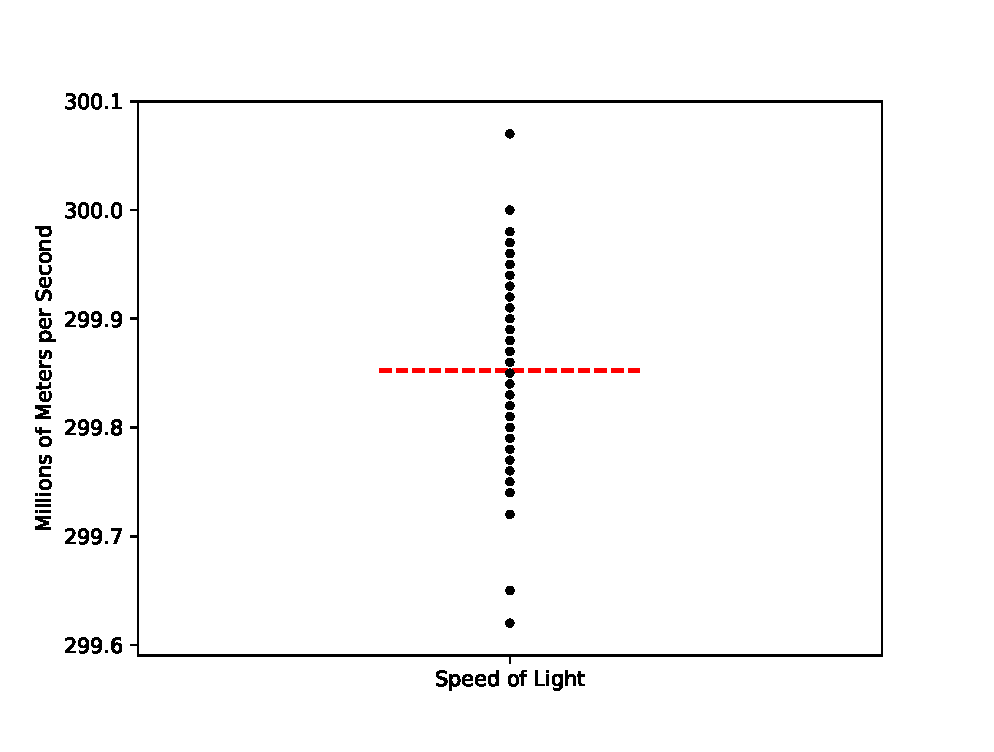
\includegraphics[width=0.85\textwidth]{./images/michelson_scatter}

  \caption{Albert Michelson's 1880 speed-of-light measurements. The mean is
    appropriate as a nominal value. The exact value is plotted for comparison.
    Visually, Michelson's mean value is `close' to the true value, though this
    begs the question `how close is close?' We can make the notion of
    `closeness' more precise by considering the variability of the data.}
  \label{fig:michelson-mean}
\end{figure}

\marginnote{Somewhat cheekily, we can note that $c = 299,792,458 m/s$ is
  \emph{exact}, as the meter is \emph{defined} in terms of the speed of
  light.\cite{thompson2008}}

While the mean is a sensible measure of central tendency, it does have some
weaknesses. We will illustrate these by contrasting against another measure of
central tendency.

\bigskip
The \emph{median}\marginnote{\underline{Definition:} The \emph{sample median} is
  the middle value of a dataset. It is a robust measure of central tendency.} is
the `middle' value of a dataset, most easily described through an example.
Suppose our data is given by $\{5, 3, 6, -1, 4\}$. We find the median by
ordering the data $\{-1, 3, 4, 5, 6\}$ and selecting the middle number; in this
case $4$. In the case where we have an even number of data points, we average
the middle two values.\footnote{e.g. $\{5, 3, 6, -1\}$ yields $\f12(3+5) = 4$}

\marginnote{Perhaps unsurprisingly, there is no universal agreement on a
  definition for the sample median. We will adopt Tukey's
  definition,\cite{tukey1977eda} but know that there are others.}

More generally, we can understand the median in terms of \emph{order
  statistics}, which are simply the ordered values of a dataset. Given our data
$X_i$, the order statistics are defined by

\begin{equation} \label{eq:def-order}
  X_{(1)} \leq X_{(2)} \leq \dots \leq X_{(n-1)} \leq X_{(n)}.
\end{equation}

\noindent The median is then given by $X_{(n/2)}$, which is simply notation for
the middle value. A definition which automatically handles the $n$ odd case is
given by

\begin{equation} \label{eq:def-sample-median}
  \tilde{X} = \f12\left(X_{(\floor{n/2})} + X_{(\ceil{n/2})}\right),
\end{equation}

\noindent where $\floor{\cdot}, \ceil{\cdot}$ define the floor and ceiling
functions. Figure \ref{fig:income-median} provides an example usage of the
median using data from the US Census Bureau. A small number of very large values
(sometimes called \emph{outliers}) can significantly impact the mean. In these
cases, the median can be a better measure of central tendency.

This being said, the mean is a more \emph{efficient} (less variable) estimator
of central tendency than the median, under particular
conditions.\cite{mosteller1977data} As we'll recommend below, one should use
multiple techniques in practice, at least when investigating a new set of data.

\begin{figure}[!ht]
  \centering
  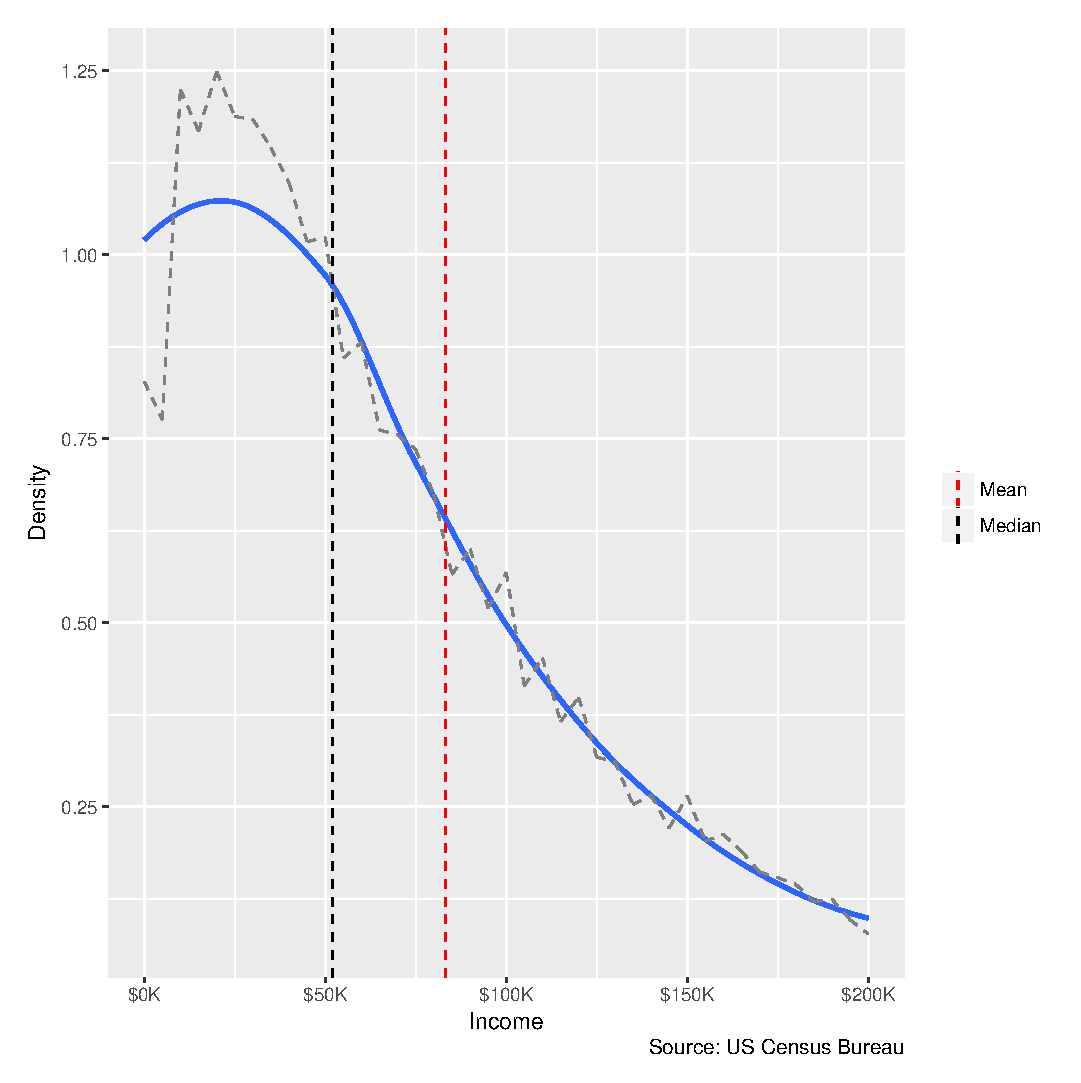
\includegraphics[width=0.85\textwidth]{./images/income}

  \caption{Distribution of sampled household incomes in the US, circa 2016.
    We'll cover density plots a bit later; but for now note that a higher
    density corresponds to a larger number of instances of that income. Notice
    that mean is pulled considerably towards higher incomes, despite the
    preponderance of lower incomes. The median is less affected by a small
    number of large values -- it is often used as a nominal value for income.
    The fact that the mean and median do \emph{not} agree here is telling -- it
    signals that something worth noting is happening in the data.}
  \label{fig:income-median}
\end{figure}

\marginnote{\underline{Concept:} \emph{Spread} is a notion of how disperse a
  distribution or data are.}

\textbf{Spread} is another apt term for a property of data. The spread is
synonymous with the variability of the data. If our data are thought to be
corrupted measurements of a true value, then spread can be thought of as the
inverse of precision. Similar to central tendency, we will introduce two notions
of spread.\footnote{In fact, in statistics lingo, \emph{precision} is inverse
  variance.}

The \emph{standard deviation}\marginnote{\underline{Definition:} The \emph{sample
    variance} is the mean-squared distance of the data from its mean. The
  \emph{sample standard deviation} is its square root. Both are measures of
  spread.} is a common measure of spread. It is defined via

\begin{equation} \label{eq:def-sample-sd}
  S = \sqrt{\frac{1}{n-1}\sum_{i=1}^n (X_i - \overline{X})^2}.
\end{equation}

Note that we must first compute the sample mean $\overline{X}$ before we can
compute $S$. Somewhat mysteriously, the denominator for $S$ is $n-1$, not $n$.
This is a subtle point that will have to wait until we introduce distributions.
For now, it will suffice to say that for small $n$, this factor\footnote{called
  the \emph{Bessel correction}} is necessary to ensure an accurate
estimate.\footnote{A bit more detail: Using the sample mean $\overline{X}$
  within $S$ causes us to loose a \emph{degree of freedom} -- a notion of
  information available from the data. We account for this `double use' of
  information through the Bessel correction.}

One may use the standard deviation to construct ranges, rather than single
values.\marginnote{A wider interval is less trustworthy than a narrow one; there
  are more true values that are compatible with the available data. However, if
  the entire interval is compatible with some conclusion -- if the interval
  itself falls within some acceptable range -- then this enables one to draw a
  more robust conclusion.} A common construction is a \emph{confidence
  interval}, which is a simple idea with some subtle points. Essentially, if
there exists a true value -- like $Y$ -- then a confidence interval will include
that value at some known \emph{confidence level}, often $95\%$ or $99\%$. An
interval gives more information than a mean alone; in addition to location, it
conveys the quality of an estimate, based on its width.

Figure \ref{fig:michelson-ci} depicts a $95\%$ confidence interval for the speed
of light, based on Michelson's 1879 data. Note that this interval includes the
true value, and gives an accurate sense of the spread of the data.

\begin{figure}[!ht]
  \centering
  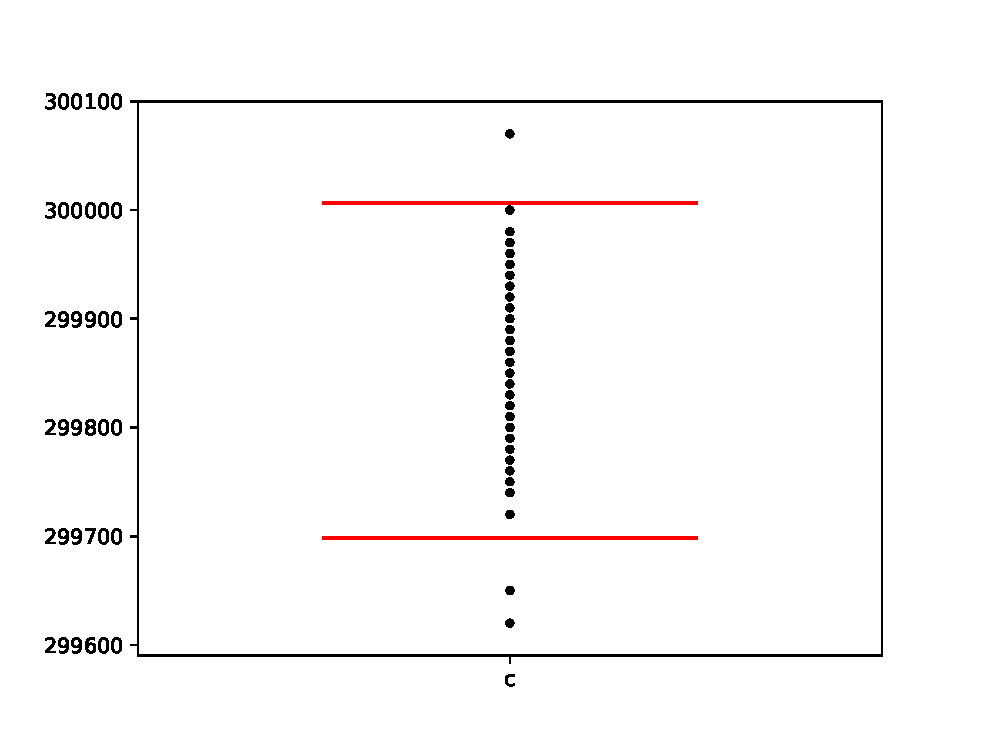
\includegraphics[width=0.85\textwidth]{./images/michelson_ci}

  \caption{Albert Michelson's 1880 speed-of-light measurements. The standard
    deviation is used to construct a confidence interval around the sample mean,
    which here includes the true speed of light. We will introduce the notion of
    \emph{confidence intervals} later when we discuss distributions.}
  \label{fig:michelson-ci}
\end{figure}

The \emph{interquartile range}\marginnote{\underline{Definition:} The
  \emph{sample interquartile range} is the distance between the sample
  quartiles. It a robust measure of spread.} (iqr) is to the standard deviation
as the median is to the mean. It is a robust measure of spread, and as its name
implies it involes the difference between \emph{quartiles} (the
quarter-quantiles) of the data. We can compute the interquartile range via

\begin{equation} \label{eq:iqr-sample}
  \text{iqr} = Q_3 - Q_1,
\end{equation}

\noindent where $Q_1$ is the median of the lower $\floor{N/2}$ of the data, and
$Q_3$ is the median of the upper fraction.\cite{tukey1977eda} The mean was
susceptible to outliers; since the variance is essentially a mean of
squared-differences, the standard deviation is similarly vulnerable to outliers.

Using the quartiles and the iqr, we can construct a \emph{boxplot}; a very
useful visual depiction of summaries. The box itself is constructed from the
quartiles of the given data ($Q_1$, the median $Q_2$, and $Q_3$), while the
lines\footnote{sometimes called \emph{whiskers} or \emph{fences}} are extended
from the quartiles by a multiple of the iqr. Points which lie outside these
extended ranges are depicted as points, and are potentially of interest.

While there are multiple versions of the boxplot,\cite{frigge1989some} all are
useful for summarizing data.

\begin{figure}[!ht]
  \centering
  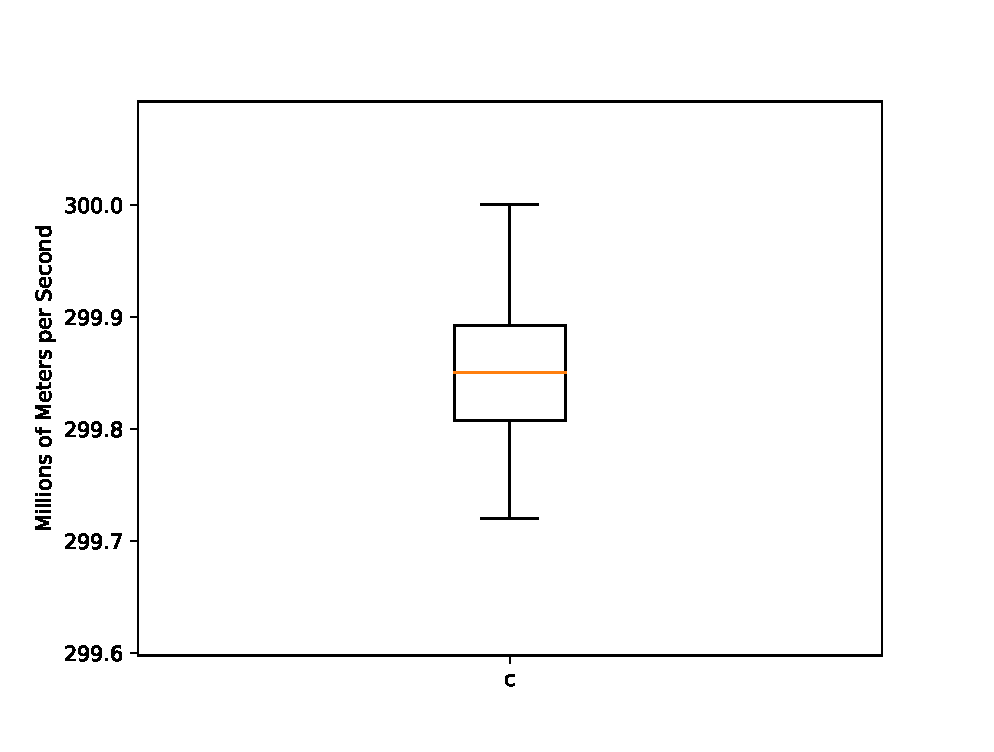
\includegraphics[width=0.85\textwidth]{./images/michelson_boxplot}

  \caption{Albert Michelson's 1880 speed-of-light measurements. The data are
    presented as a boxplot, which highlights a number of potential outliers.}
\end{figure}

\textbf{Correlation} is important for studying the relationship between
variables. Correlation is defined for two random variables $\mX,\mY$ via

\begin{equation} \label{eq:corr-pearson}
  \rho_{\mX,\mY} = \frac{\text{Cov}(\mX,\mY)}{\sigma_{\mX}\sigma_{\mY}},
\end{equation}

\noindent where $\text{Cov}(\mX,\mY)\equiv\E[(\mX-\E[\mX])(\mY-\E[\mY])]$ is the
covariance between $\mX,\mY$, and the $\sigma$ are their standard deviations. In
truth \eqref{eq:corr-pearson} is called the \emph{pearson correlation}, to
distinguish it from other correlation definitions. Pearson correlation measures
\emph{linear} correlation between quantities; it well tend to fail to find
nonlinear relations between variables.

\begin{figure}[!ht]
  \centering
  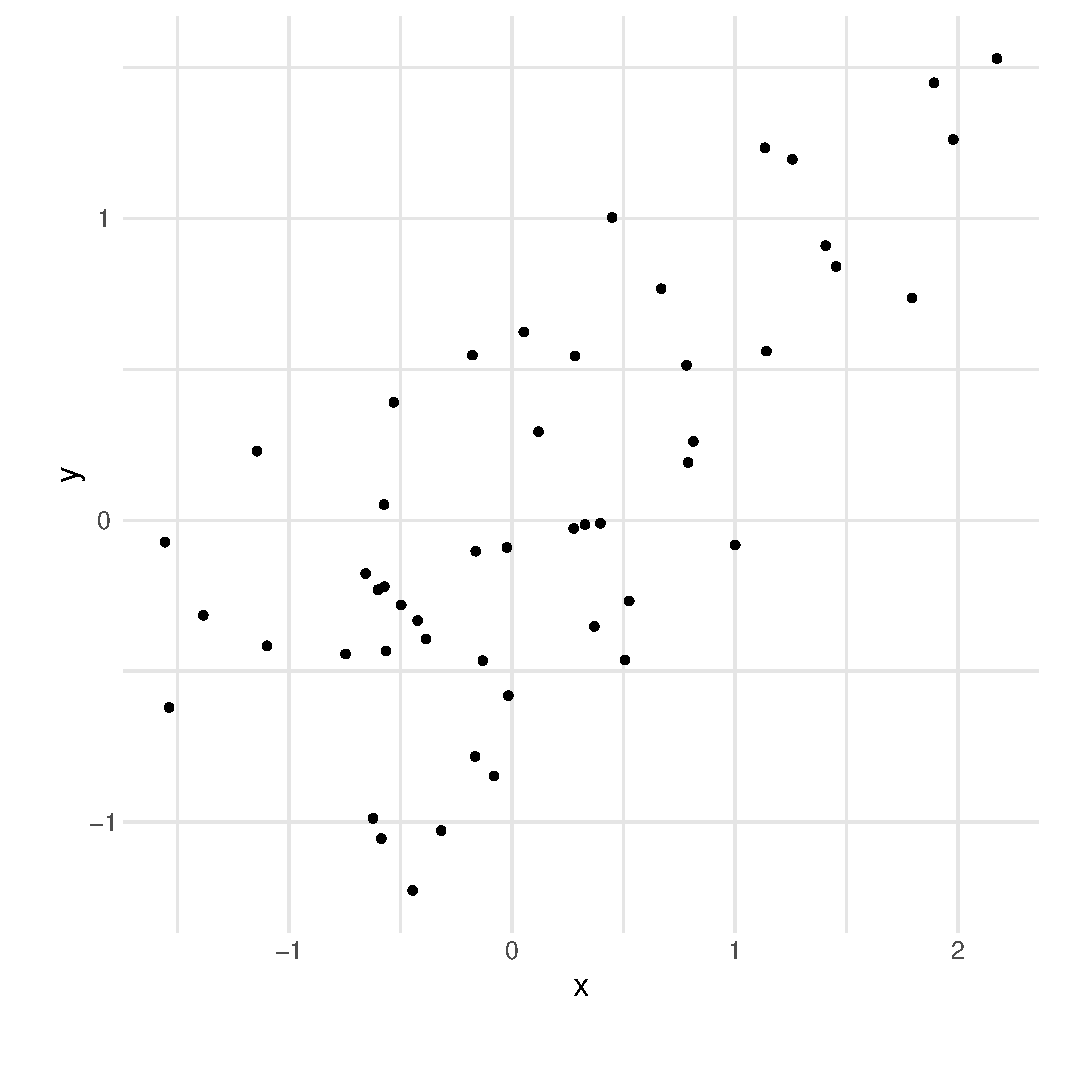
\includegraphics[width=0.85\textwidth]{./images/corr_xy}\\
  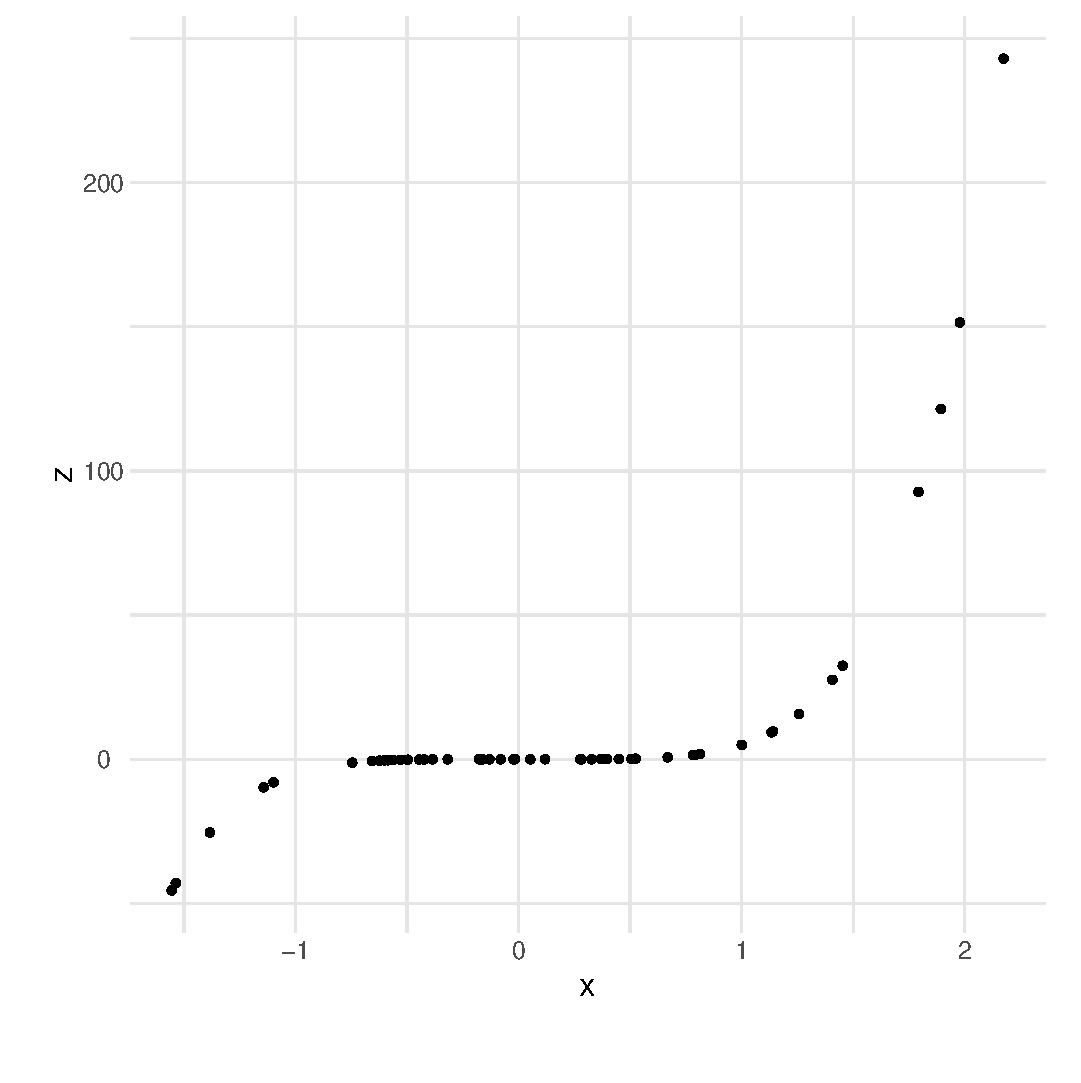
\includegraphics[width=0.85\textwidth]{./images/corr_xz}

  \caption{Example data used for demonstrating correlation. The top case has a
    true underlying correlation of $\f12$; with these $50$ data points the
    pearson correlation is $\rho_{\mX,\mY} = 0.719$, and the spearman
    correlation is $r_{\mX,\mY} = 0.661$. The bottom case has a perfect
    monatonic relation; with these $50$ data points the pearson correlation is
    $\rho_{\mX,\mY} = 0.711$, and the spearman correlation is $r_{\mX,\mY} =
    1.0$.}
\end{figure}

An alternative formulation is \emph{spearman's rho} or \emph{spearman
  correlation}, which is defined as the pearson correlation between \emph{rank
  variables}

\begin{equation}
  r_{\mX,\mY} = \rho_{R_{k,\mX},R_{k,\mY}}
\end{equation}

\noindent where \emph{rank variables} $R_{k,\mX},R_{k,\mY}$ are simply the
indices of the ordered observations of $\mX$ and $\mY$, much like computing
order statistics.\cite{conover1980practical}

\textbf{Skepticism} is vitally important when analyzing data. In practice, one
should be skeptical both of the data, \emph{and} of the techniques used to
analyze the data.

\emph{Techniques} are vulnerable to faulty assumptions -- when analyzing data,
one should employ multiple methods and compare their results.
Tukey\cite{tukey1979robust} stated this quite directly when he wrote

\begin{quote}
It is perfectly proper to use both classical and robust/resistant methods
routinely, and only worry when they differ enough to matter. BUT when they
differ, you should think HARD.
\end{quote}

This is why we covered both classical (mean, standard deviation) and robust
(median, iqr) summaries -- in practice, you should use both, at least when first
studying a new dataset. This will enable you to catch features of the data that
might otherwise go undetected, such as the difference between the mean and
median in the Census data above.

Data are also vulnerable to errors, and may contain outliers. When first
studying a new dataset, one should first check for these sorts of problems.
Common approaches include checking for impossible values (e.g. zero-width
measurements of a diamond) or gross outliers (for which a boxplot is very
helpful).

More broadly, one should engage in \emph{exploratory data analysis} (EDA) before
proceeding with more analytical investigations.\cite{tukey1977eda} This is a
crucial step where one seeks to understand the data, especially to check
assumptions that subsequent analyses may rest upon. However, EDA is a broad
subject, beyond the scope of this primer.

\subsection{Distributions}
%% -------------------------
We will use distributions to model uncertain quantities. A \emph{distribution}
defines a \emph{random variable} $X$ -- an uncertain quantity which takes
(potentially) different values upon different observations. Some examples of
physical phenomena we might model with a random variable include: the outcome of
a coin flip, the roll of a twenty-sided die, the ambient temperature in New York
City, the thrust output of a jet engine subject to uncertain inlet conditions.
Note that some of the preceding examples are discrete (the coin and die), while
the others are continuous (temperature and thrust). While discrete random
variables certainly have their applications, we will focus on continuous
distributions.

Why would we bother modeling uncertain quantities? In cases where we have data,
we can use a model to do \emph{inference}. Suppose our random variable model
arises from a physical argument, and its fitted parameters have some physical
meaning. In this case, fitting the model is an exercise in learning physical
properties about the process which generated the data, much like the barometer
example above. We will introduce a simple way to fit distributions below.

In cases where we have no data, but can make informed statements about what the
data \emph{might} look like were we to observe them, we can use distributions to
make these statements quantitative.

Formally, a distribution is a \emph{function} which describes how likely a
random variable is to take a particular value. Figure \ref{fig:dist-norm}
provides an illustrative example through displaying the standard normal's
\emph{probability density function} (PDF) and \emph{cumulative density function}
(CDF). Both functions convey the same information, but in different forms; the
PDF can be interpreted as describing the \emph{likelihood} of a single value
$x$, while the CDF can be interpreted as describing the \emph{probability} of
observing a value at most equal to $x$.\footnote{The distinction between
  likelihood and probability is important for continuous random variables;
  technically, any single value $x$ that a random variable $X$ might take has
  \emph{zero probability}, but a possibly-finite likelihood.}

\begin{figure}[!ht]
  \centering
  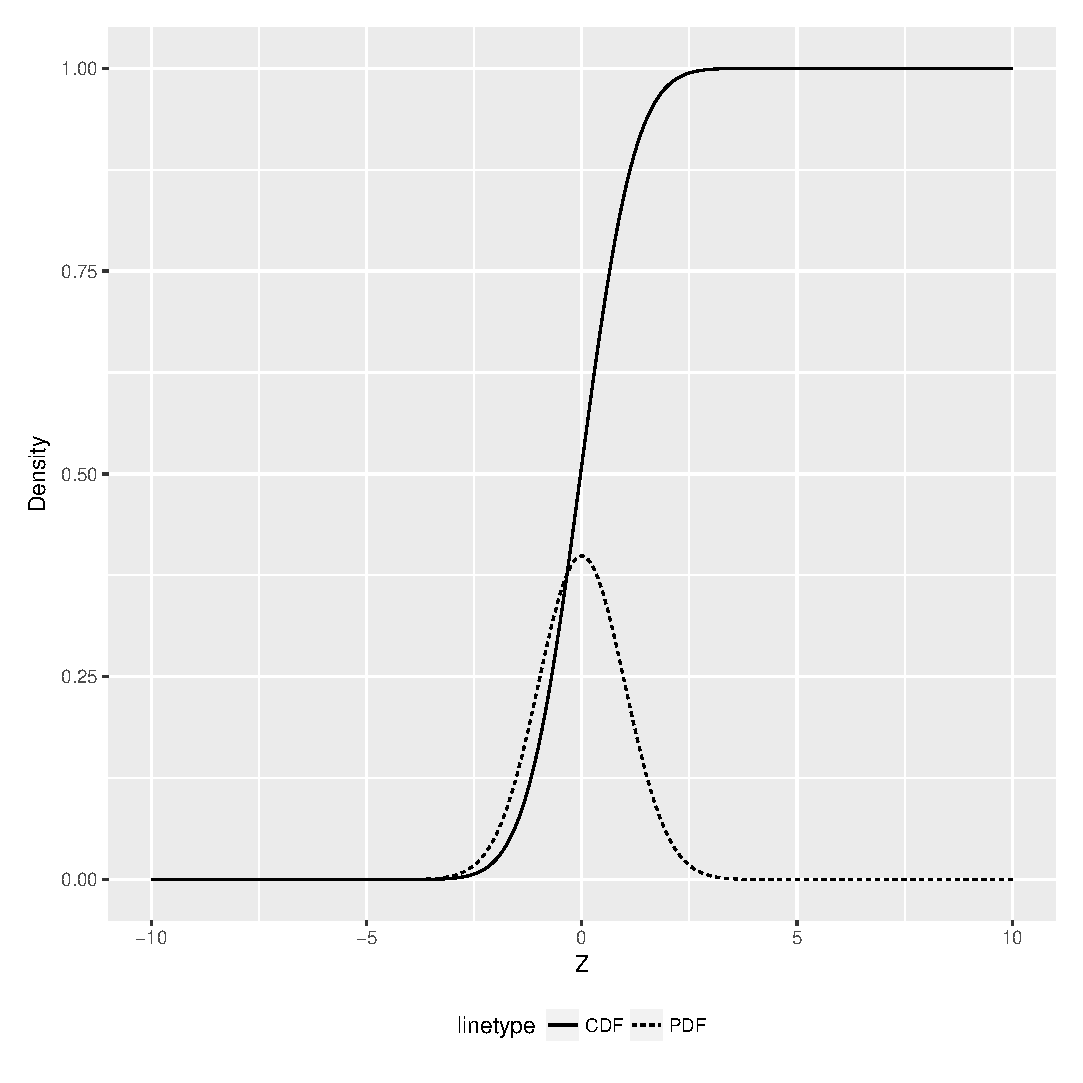
\includegraphics[width=0.85\textwidth]{./images/dist_normal}

  \caption{Standard normal distribution PDF and CDF. Note that higher values of
    the PDF correspond to more likely values for the associated random variable;
    thus, this density's most likely value is zero. The CDF shows us that values
    below $Z\approx-2.5$ are highly improbable.}
  \label{fig:dist-norm}
\end{figure}

More formally, the CDF $F_X(x)$ for a continuous random variable $X$ is the
function that returns the probability of observing a result \emph{at least} as
extreme as a test value $x$, that is

\begin{equation} \label{eq:ch3-def-cdf}
  F_X(x) = \P[X \leq x].
\end{equation}

\noindent The PDF $f_X(x)$ is the derivative of the CDF, that is

\begin{equation} \label{eq:ch3-def-pdf}
  f_X(x) = \frac{d F_X}{dx}.
\end{equation}

\noindent Points $x$ with greater values $f_X(x)$ are more likely to occur.
Distributions contain quite a bit of information; one way to summarize
distributions is to compute an \textbf{expectation}. The expectation is a linear
operator on a random variable defined via

\begin{equation} \label{eq:ch3-def-expectation}
  \E[\phi(X)] = \int \phi(x) f_X(x) dx.
\end{equation}

\noindent Different choices of function $\phi(\cdot)$ allow us to express many
useful quantities; for instance, by the definition of the CDF, we can write

\begin{equation}
  \P[X \leq x] = \E[\i1_{x' | x' \leq x}(x)],
\end{equation}

\noindent where $\i1_{S}(\cdot)$ is the \emph{indicator function}, which
indicates whether a point is within a given set $S$ via

\begin{equation}
  \i1_{S}(x) = \left\{\begin{array}{ll} %
    1 & x \in S \\
    0 & x \not\in S
  \end{array}\right.
\end{equation}

When using distributions for modeling, we assume that data are generated by some
underlying process which has some distribution -- we call this a
\emph{population}. Data drawn from this population are called a \emph{sample}.
This distinction allows us to clarify the difference between the sample
summaries we considered above, and the \emph{moments} we consider now.

\noindent\textbf{Moments} are properties of a distribution, and are directly
connected to the summaries introduced above. While sample moments summarize a
dataset, the moments we consider here summarize an entire function -- a
distribution. Familiar moments include the mean $\mu$ and variance $\sigma^2$,
defined

\begin{equation} \begin{aligned} \label{eq:ch3-common-moments}
    \mu      &\equiv \E[X], \\
    \sigma^2 &\equiv \E[(X-\E[X])^2], \\
             &= \E[X^2] - \E[X]^2,
\end{aligned} \end{equation}

\noindent These are exact moments for a given distribution; we may regard the
sample mean and sample variance introduced above as \emph{approximations} to
these true values.\footnote{Formally, assuming the existence of true moments or
  parameter values is a \emph{frequentist} philosophy, in contrast with a
  Bayesian perspective.} The difference between a sample moment computed from an
observed sample and the true moment is a form of \emph{sample error}, and is one
form of uncertainty we might seek to quantify. Assuming a distribution for an
underlying population will help us to do this, but keep in mind that our results
will only be as trustworthy as our assumptions!

Since moments are in effect summaries of distributions, two distributions may
share a few moments in common, and yet have a completely different shape. The
choice of data-modeling distribution is informed by this additional information
-- we will introduce a few important distributions, and provide brief commentary
on others.

\noindent\textbf{Uniform Distribution}

The uniform distribution is often used to encode constraints; if a value is
known (or asserted) to lie between some bounds, the uniform distribution puts
equal likelihood on every point between those bounds.

We denote a random variable drawn from a uniform distribution with bounds $a<b$
via

\begin{equation}
  U \sim U[a,b].
\end{equation}

\noindent\textbf{Normal Distribution}

We denote a random variable drawn from a normal distribution with mean $\mu$ and
variance $\sigma^2$ via

\begin{equation}
  X \sim N(\mu, \sigma^2).
\end{equation}

\noindent If $\mu=0$ and $\sigma^2=1$, then the associated normal is called
\emph{standard}, and is often denoted $Z \sim N(0, 1)$. Note that if we know the
true mean and variance, we can always standardize a normal random variable $X$
via

\begin{equation}
  \frac{X - \mu}{\sigma} \sim N(0, 1).
\end{equation}

The normal distribution is extremely common as an assumed distribution. This
assumption is endorsed by the central limit theorem, which gives the normal as
the limit distribution for sums of random variables, meeting certain technical
conditions.\cite{van1998asymptotic} For example, if we have a set of data $X_i$
for $i=1,\dots,n$ where each of the $X_i$ are drawn from the same population
with finite mean and variance, then as $n\to\infty$, we find

\begin{equation} \label{eq:mean-clt}
  \overline{X} = \frac{1}{n}\sum_{i=1}^n X_i \stackrel{d}{\to} N(\E[X], \V[X]/n),
\end{equation}

\noindent where $\stackrel{d}{\to}$ denotes convergence in distribution -- a
particular (weak) form of convergence. Note that while $X$ \emph{may not be
  normal}, the sample mean converges to a normal distribution centered around
the true mean $\E[X]$. Note also that the variance of this asymptotic
distribution scales as $1/n$; thus the standard deviation scales as
$1/\sqrt{n}$.

The normal distribution $N(\E[X], \V[X]/n)$ is called the \textbf{sampling
  distribution} for the estimator $\overline{X}$; this distribution will be
useful later when we define \emph{confidence intervals}. The standard deviation
of the sampling distribution -- in this case $\sigma/\sqrt{n}$ -- is called the
\textbf{standard error} of the estimate, and is a measure of the noise in our
estimate.

\noindent\textbf{Chi-Squared Distribution}

The sample mean is asymptotically normal under fairly generous conditions; can
we make a similar statement about the sample variance? The sample variance is
also a sum of random variables,\footnote{Recall $S^2 = \sum_{i=1}^n (X_i -
  \overline{X})^2$} but these may not be independent. \emph{However}, in the
case where $X$ is (exactly) normally distributed, the terms in the sample
variance \emph{are} independent. In this case, each term is an independent,
squared, standard normal random variable, which we denote

\begin{equation} \label{eq:chi-squared}
  \chi^2_{\nu} = \sum_{i=1}^{\nu} Z_i^2,
\end{equation}

\noindent and call a \emph{chi-squared} random variable with $\nu$ \emph{degrees
  of freedom}. One may show that

\begin{equation} \label{eq:sample-dist-var}
  S^2 \sim \sigma^2 \chi^2_{n-1} / (n-1),
\end{equation}

\noindent which is the sampling distribution for $S^2$, \emph{assuming} $X$ is
exactly normal. \textcolor{red}{TODO} Bessel's correction?

\noindent\textbf{Student's t Distribution}

The chi-squared distribution is constructed from squared normals. In the case
where $X$ is exactly normal, we may use the sample mean and variance to
construct a normalized quantity, which can be expressed in terms of the ratio of
an independent standard normal and chi-squared variables

\begin{equation} \label{eq:t-def}
  \frac{\overline{X} - \mu}{S/\sqrt{n}} = \frac{Z}{\sqrt{\chi^2_{n-1}/(n-1)}} \equiv t_{n-1},
\end{equation}

\noindent where $t_{n-1}$ follows \emph{Student's t distribution} with $n-1$
degrees of freedom. Contrast Student's t with the standardization of a
non-standard normal

\begin{equation}
  \frac{\overline{X} - \mu}{\sigma/\sqrt{n}} \sim N(0, 1).
\end{equation}

Student's t is important for \emph{hypothesis testing}; we introduce it here to
discuss the important concept of \emph{tail behavior}. The top panel of Figure
\ref{fig:dist-sheet} contrasts some example Student's t distributions against a
standard normal; note that -- in comparison with a gaussian -- Student's t
distribution is slower to decay to zero as one goes to $\pm\infty$. It is for
this reason that Student's t is said to have \emph{heavy} tails, compared to a
normal distribution.

Mosteller and Tukey\cite{mosteller1977data} discuss ways in which a distribution
can be nonnormal, and note that tail behavior tends to be both the hardest to
detect and the most consequential. Heavy tails imply that large values -- values
far from the center of the distribution -- tend to occur more frequently than we
might expect from a similar normal distribution. As Mosteller and Tukey note
this can ``alter a sample mean drastically, and a sample $S^2$
catastrophically!'' In practice, if a real process is suspected to exhibit heavy
tails, a t distribution may be a more appropriate model than a normal.

Figure \ref{fig:dist-sheet} depicts the distributions described above, for a
number of different parameters, and with their first two moments described in
terms of their parameters.

\begin{figure*}[!ht]
  \centering
  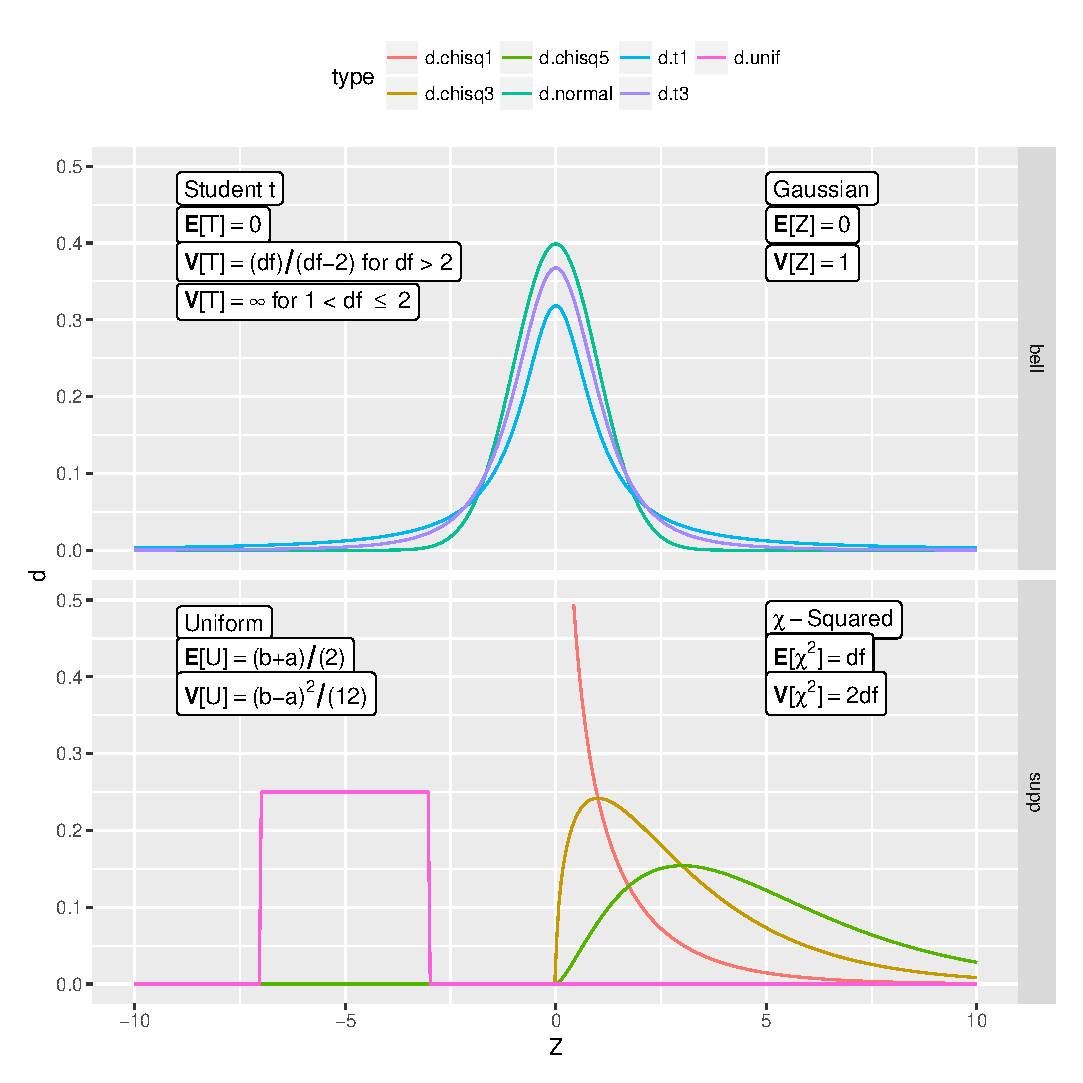
\includegraphics[width=0.85\textwidth]{./images/dist_sheet}

  \caption{Common densities and their first two moments. Note the heavy tails of
    the t distributions, and the shifting central tendency of the chi-squared
    distribution with increasing degrees of freedom.}
  \label{fig:dist-sheet}
\end{figure*}

\noindent\textbf{Other Distributions} \textcolor{red}{TODO} A list and brief
commentary on other distributions.

\noindent\textbf{Lognormal Distribution}

\noindent\textbf{Weibull Distribution}

\noindent\textbf{F Distribution}

\noindent\textbf{Matching Moments} is a simple way to fit a distribution to
data. For a normal distribution this is easy, as it is parameterized in terms of
its mean and variance -- given data, we could easily compute the sample mean and
variance, and construct a normal distribution that matches these estimated
moments. This is not necessarily a good idea; suppose the moment estimates were
quite noisy (have high standard error) -- this additional variability would not
be accounted by simply matching moments.

These difficulties are compounded by the inherent difficulty in estimating
higher-order moments. While the normal distribution is defined by its mean and
variance alone, other distributions have more parameters to fit. In general,
higher-order moments -- larger exponents in $\E[X^k]$ -- are more difficult to
estimate. This is because we loose \textbf{degrees of freedom} in the data by
estimating the lower-moments. Recall that the sample mean $\overline{X}$ appears
in each term of the sample variance;\footnote{given by $S^2 = \sum_{i=1}^n (X_i
  - \overline{X})^2$} we have used the data to estimate the quantity
$\overline{X}$, and have lost some available information in doing so. This
notion of information is made formal in the degrees of freedom, which can be
understood in terms of the dimension of the subspace spanned by the data --
computing the sample mean essentially introduces a constraint, which reduces the
dimension of the data available for the variance by one. This reduction reduces
the effective sample size to $n-1$, which is captured in the Bessel correction,
and points to the difficulty in estimating the variance, relative to the mean.
Higher moments compound this difficulty with further reduction in degrees of
freedom.

The difficulty in estimating higher moments is closely related to tail behavior,
and is a fundamental issue. For instance, the kurtosis $\text{Kurt}[X] =
\E\left[\left(\frac{X - \mu}{\sigma}\right)^4\right]$ is a fourth-order moment,
commonly used to describe tail behavior -- a kurtosis greater (or smaller) than
that of a similar normal distribution points to heavier (or lighter) tails.

Finally, note that a chosen distribution introduces \emph{additional}
information beyond the fitted moments, in particular fixing higher-order moments
in terms of the parameters. For instance, assuming a normal vs Student's t makes
an assertion about tail behavior, and both assume a symmetric distribution.
Modeling a random quantity requires careful thought about what behavior it may
exhibit, and should ideally be supported by both data and relevant knowledge.

As a side note, an alternative to matching moments is to fit distribution
parameters -- and account for their uncertainty -- via some inferential
procedure. We will discuss \emph{predictive distributions} in Chapter
\ref{ch:wrangle} Section \ref{sec:inverse-propagation}.

\textbf{Confidence Intervals} are a common way of expressing uncertainty about
an estimated quantity. In contrast with reporting a single estimated value -- a
\textbf{point estimate} -- a confidence interval brackets the true quantity to
be estimated, at a desired \emph{confidence level} -- a probability of
containing the true value. Note that the confidence in this framework is in the
\emph{procedure that generates the interval}, and \emph{not in the interval
  itself}.\footnote{Confidence intervals are frequentist constructions, which
  rely on the assumption that there exist true values to be estimated. Under
  this assumption, any given interval either does or does not include the true
  value. Thus, the associated confidence needs to be understood as a property of
  the process that generated the interval, and not a particular given interval
  itself.}

For example, it is common to seek confidence intervals for mean estimates, which
gives a sense of how trustworthy an estimate is -- a `wide' interval indicates
that one is not very certain about the estimate. Note that the sample mean
(under appropriate assumptions) is asymptotically normal;\footnote{with
  $\overline{X} \sim \dN(\mu, \sigma^2/n)$} one can use this limiting behavior
to construct \emph{approximate} confidence intervals. If we happened to have the
exact variance (which never happens in practice), we could define a symmetric
confidence interval around a given sample mean at a desired confidence level
$C\in[0,1]$ via

\begin{equation} \label{eq:mean-ci}
  [\overline{X} - z_C \sigma, \overline{X} + z_c \sigma],
\end{equation}

\noindent where $z_c = - \Phi^{-1}(\frac{1-C}{2})$, and $\Phi^{-1}(\cdot)$ is
the standard inverse normal CDF. In the case where $\overline{X}$ was exactly
normal, \Cref{eq:mean-ci} would have the desired coverage probability. However,
if $\overline{X}$ were only asymptotically normal this would not be the case,
but the realized coverage probability would approach the desired as one drew
more samples. Note that in practice, we would would need to use the sample
standard deviation $S$ in place of the unknown $\sigma$, which would introduce
another level of approximation. In the case where $n$ is small, say $n < 10$, it
may be prudent to account for this additional approximation by using Student's t
distribution.\footnote{One could do this by using a $t_c$ value in place of
  $z_c$, choosing from the inverse t CDF with appropriate degrees of freedom $df
  = n - 1$.}

\subsection{Manipulating random variables}
%% -------------------------
Some basic understanding of how random variables interact is useful for hand
calculations (useful for verifying stochastic codes) and for building intuition.
We'll review a few simple calculations for random variables here.

\textbf{Moment manipulations} are extremely common for random variables. Linear
operations are particularly fundamental.

\textbf{Exercise:} Using \eqref{eq:ch3-def-expectation}, show that $\E[a + bX] =
a + b \E[X]$.

\textbf{Exercise:} Using \eqref{eq:ch3-def-expectation} and
\eqref{eq:ch3-common-moments}, show that $\V[a + bX] = b^2 \V[X]$.

The situation is a bit more complicated when multiple random variables are
involved.

\textbf{Exercise:} Using \eqref{eq:ch3-def-expectation}, show that $\E[aX_1 +
  bX_2] = a \E[X_1] + b \E[X_2]$.

\textbf{Exercise:} Using \eqref{eq:ch3-def-expectation} and
\eqref{eq:ch3-common-moments}, show that $\V[aX_1 + bX_2] = a^2 \V[X_1] + b^2
\V[X_2] + 2ab \Cov[X_1,X_2]$.

\textbf{Gaussian manipulations} are very useful, in part because they are
tractable for hand calculations. One of the \emph{fundamental facts} about a
gaussian is that it is fully defined by its mean and variance.

\textbf{Exercise:} Let $X_1\sim\dN(\mu_1, \sigma_1^2), X_2\sim\dN(\mu_2,
\sigma_2^2)$. Show that

\begin{equation} \label{eq:ch3-add-normal}
  a X_1 + b X_2 \sim \dN(a \mu_1 + b \mu_2, a^2 \sigma_1^2 + b^2 \sigma_2^2).
\end{equation}

\noindent \Cref{eq:ch3-add-normal} shows us that while the central tendencies of
gaussians adds, their \emph{standard deviations do not add}. This seemingly
trivial result actually defies the common engineering intuition, and provides a
very simple motivation for propagating uncertainty `properly'.

Suppose a structural engineer were designing a simple member to carry a uniaxial
load for an aircraft. According to the \emph{legal} requirements for aircraft
airworthiness, the designer must use a quantile estimate\footnote{technically a
  \emph{basis value}, required by Title 14 CFR 25.613} for material properties.
This is to account for manufacturing variabilities; for a concrete example,
suppose the yield strength of the material is distributed according to
$\Sigma\sim\dN(\mu_{\Sigma}, \sigma_{\Sigma}^2)$, and the applied load is also
uncertain, following $F\sim\dN(\mu_F, \sigma_F^2)$. Given a fixed
cross-sectional area $A$ to carry the load, the probability of failure of the
structure is

\begin{equation} \label{eq:ch3-tension}
    \P[ \Sigma < F/A ] = \Phi\left( %
      \frac{\mu_{\Sigma} - \mu_F/A}{\sqrt{\sigma_{\Sigma}^2 + \sigma_F^2/A^2}}
    \right).
\end{equation}

\noindent The quantile of $\Sigma - F/A$ relevant to achieving a desired failure
probability $p_f$ is given by

\begin{equation} \label{eq:ch3-lim-quantile-true}
  g_{\text{true}} = (\mu_{\Sigma} - \mu_F/A) + %
    \Phi^{-1}(p_f)\sqrt{\sigma_{\Sigma}^2 + \sigma_F^2/A^2}.
\end{equation}

However, \emph{first} computing input quantiles -- separately, at the $p_f$
level -- and \emph{then evaluating} those fixed values yields the value

\begin{equation} \label{eq:ch3-lim-quantile-eval}
  g_{\text{eval}} = (\mu_{\Sigma} - \mu_F/A) + %
    \Phi^{-1}(p_f)(\sigma_{\Sigma} + \sigma_F/A).
\end{equation}

One can understand the current industrial practice as solving $g_{\text{eval}} =
0$ for $A$.\footnote{The true industrial practice is actually a bit more
  conservative than this, as basis values account for epistemic sampling
  uncertainty, in addition to the aleatory manufacturing uncertainty.} The
consequence of \emph{not propagating uncertainty} is to expose oneself to the
unknown discrepancy $g_{\text{true}} - g_{\text{eval}} \neq 0$. Without
rigorously quantifying the uncertainty -- even for this simple linear function
-- one cannot control probabilities of failure.

\textbf{Exercise:} Derive \eqref{eq:ch3-tension} using property
\eqref{eq:ch3-add-normal}.

\textbf{Exercise:} Suppose a designer solves $g_{\text{eval}} = 0$ for $A$ under
a desired value of $p_f < 0.5$. How does the true value $\P[ \Sigma < F/A ]$
compared to the designed value $p_f$?

\textbf{Exercise:} Assess the appropriateness of the random variable model
proposed above for $\Sigma$ and $F$; is the model reasonable, both from a
physical and practical standpoint? What are its merits and failings?

While independent gaussians are simple to manipulate, the case is somewhat more
complicated for \emph{correlated} normal variables. If two or more variables are
correlated, one must consider their \emph{joint} density. For a vector of normal
variables $\mX\in\R{d}$ this is reasonably easy to handle; suppose $\mX \sim
\dN(\v\mu, \m\Sigma)$, where $\v\mu\in\R{d}$ is the vector mean, and
$\m\Sigma\in\R{d\times d}$ is the covariance matrix. For the distribution to be
valid, we must have $\m\Sigma$ positive semi-definite \footnote{positive
  semi-definite is often denoted $\m\Sigma\geq0$; that is for all $\vx\in\R{d}$,
  we have $\vx^{\top}\m\Sigma\vx \geq 0$.} and $\m\Sigma^{\top} = \m\Sigma$. We
can handle a linear combination of correlated normals by a transformation to
uncorrelated normal variables.

Let $\m\Sigma^{\f12}$ be the \emph{Cholesky decomposition} of $\m\Sigma$,
satisfying

\begin{equation}
  \m\Sigma = \left(\m\Sigma^{\f12}\right)^{\top} \m\Sigma^{\f12},
\end{equation}

\noindent where $\m\Sigma^{\f12}$ is unique. Then $\mX$ is distributed the same
as $\v\mu + \left(\m\Sigma^{\f12}\right)^{\top}\mZ$ with $\mZ\sim\dN(\v0, \mI)$.

\textbf{Exercise:} Using property \eqref{eq:ch3-add-normal}, show that $\mX' =
\v\mu + \left(\m\Sigma^{\f12}\right)^{\top}\mZ$ has the distribution $\dN(\v\mu,
\m\Sigma)$.\footnote{Hint: It suffices to show that $\E[\mX'] = \v\mu$ and
  $\V[\mX'] = \m\Sigma$, as a gaussian is fully defined by its first two
  moments.}



%% --------------------------------------------------
\section{Interval Characterization} \label{sec:intervals}
%% --------------------------------------------------

%% --------------------------------------------------
\section{Models} \label{sec:models}
%% --------------------------------------------------
Scientists and engineers use models to answer questions. Scientists build models
to encode hypotheses relating physical quantities, then gather data to test
these hypotheses, in order to come to a fuller understanding of the physical
world. Engineers build predictive models to simulate physical processes, in
order to support the design of systems.

Above, we used distributions to model uncertain quantities; here, we will
discuss means to model \emph{relationships between quantities}. We will briefly
discuss different means to do this -- using either physics or data -- then focus
on how to assess models with regard to uncertainty, introducing the notion of
\emph{sensitivity analysis}, and detailing some methods and their usage.

To keep a consistent nomenclature, here and throughout we will consider models
which take some deterministic input $\vx \in \cD \subseteq \R{m}$ in a domain
$\cD$, and return a single, deterministic, scalar output $y \in \R{}$, with the
functional relation

\begin{equation}
  y = f(\vx).
\end{equation}

\noindent Note that we may have multiple output quantities of interest $y_i$,
which arise from multiple functions $f_i(\vx)$; however, not all techniques we
will study generalize well to vector outputs, so we will primarily consider
scalar outputs.

\subsection{Kinds of Models}
%% -------------------------
Scientists and engineers often derive \textbf{models from physics}; i.e. from
physical principles and laws. These relations are derived under particular
assumptions, and thus are only as accurate as their assumptions.

For instance, Newton's laws form a good model for the dynamics of rigid bodies
at human length- and time-scales. From this set of simple rules, one can derive
equations of motion which can be solved for the dynamics of a system. Stepping
up in complexity, many scientific and engineering models are expressed as
partial differential equations, which form a map between the input parameters
$\vx$ -- expressing boundary conditions, geometries, material properties and so
on -- and the outputs $\vy$ -- expressing resulting stresses, displacements,
flow fields, trajectories, and so on.

Many physical laws involve constants that are fitted from physical data; for
instance, Newton's laws introduce mass as a constant of proportionality between
force and acceleration. The laws create a mapping from these (possibly fitted)
values to the output quantities of interest, such as the trajectory of a rigid
body. The physical laws will often include other inputs of interest, such as a
time duration ahead of some starting condition, or a location in space.

In the classical dynamics setting, the inputs $\vx$ might include the masses of
objects, initial positions, and a time of interest, while $y$ might be the
position of a particular body at the time of interest. These inputs, and their
dependent predictions, are usually thought to be determinstic under physical
laws.\footnote{Some notable exceptions include quantum mechanics and statistical
  mechanics.} For a single input $\vx$, we obtain a unique value $y$.

However, in many practical cases, the inputs $\vx$ are not known exactly, but
are uncertain. The inputs may be `genuinely' random, or may simply not be fully
characterized. In either case, it is common to model this uncertainty on the
inputs as a multivariate random variable $\mX$. In this case, the mapping
$f(\vx)$ creates a new random variable $Y = f(\mX)$, with randomness induced by
the uncertain inputs $\mX$, and transformed by the model arising from physics.
This leads to a very practical question: ``Is the uncertainty in $Y$
significant?'' The answer to this question depends both on how uncertain we are
about $Y$, and for what purpose we intend to use this information. The latter
depends on problem formulation, while the former falls under the purview of
uncertainty propagation.

For instance, the gravitational constant $G$ is necessary for studying problems
in celestial mechanics. Some measurements of $G$ have uncertainty on the order
of 150 parts per million.\cite{rosi2014precision} Even without elaborate
uncertainty propagation, it seems reasonable that this level of uncertainty
would not pose a serious challenge to launching satellites to orbit. However,
the same measurement above disagrees with the accepted\footnote{by the Committee
  on Data for Science and Technology} value of $G$ by $1.5$ standard deviations
-- repeated instances of measurements differing by this amount would be of
concern from a scientific perspective.

Scientists and engineers also derive \textbf{models from data}, which share many
of the same characteristics as models from physics. Such data-driven models also
provide a mapping from inputs to outputs, enabling prediction. However, models
from physics are \emph{conceptual} as well as \emph{quantitative}; Newton's laws
enable one to \emph{understand} motion in the language of forces and
accelerations. A curve fitted to trajectory data lacks this richness of
interpretation.

While physics allows one to peek `under the hood' of a physical system, data
driven models have the potential to step outside human limits. In cases where
the physics are poorly understood -- and appropriate data is available -- one
can use a data driven approach to model phenomena and solve problems. A data
driven approach can also -- in principle -- scale to arbitrary problem size,
assuming sufficient computation and information are available. In cases when
pragmatism is valued, data driven approaches can be very appropriate.

Note that `data driven' does not necessarily mean `automatic,' or that knowledge
of (and respect for) the underlying physical phenomena is not necessary for
success. Building data driven models is a challenging task to do well, requiring
both statistical, engineering, and domain knowledge. We will cover regression --
a particular data driven approach -- in a following chapter.

Finally, we note that the distinction between models from physics and data is,
at least philosophically, somewhat arbitrary. All physical laws are in some way
derived from observations of the physical world. However, commonly accepted laws
have generally been subjected to extensive testing, and have survived attempts
at falsification.\cite{popper2005logic} Physical laws represent our best
understanding of the physical world to date, and therefore are usually more
trustworthy than models derived from a particular dataset.

Where the distinction above becomes (actionably) useful is in realizing that
models tend to be more trustworthy for simpler, more-extensively tested
settings. Newton's laws provide an extremely accurate model for projectile
motion. One could derive a \emph{stock and flow model} for ecological dynamics
under conservation principles, but the analyst would need to account for all
manner of sinks, sources, and interactions between species and the environment.
Pilkey and Pilkey-Jarvis\cite{pilkey2007useless} provide numerous negative
examples in environmental science, and warn against unwarranted trust in such
models.

However, as scientists and engineers, we would like to progress from simple,
well-understood cases towards more complicated settings of interest. How can we
confidently build from first principles and data towards a useful model? A key
step in building trust in a model is \emph{validation}.

\subsection{Validation}
%% -------------------------
\textbf{Validation} is a key step in model building, and is one of the core
motivations behind performing uncertainty quantification. Validation is often
paired and discussed alongside \textbf{verification}. We present the AIAA
definitions of verification and validation, by way of Oberkampf and
Barone.\cite{oberkampf2006measures}

\textbf{Verification} is: The process of determining that a model implementation
accurately represents the developer's conceptual description of the model and
the solution to the model.

\textbf{Validation} is: The process of determining the degree to which a model
is an accurate representation of the real world from the perspective of the
intended uses of the model.

Both are exercises in determining correctness, but \emph{verification} is an
exercise in \emph{software}, while \emph{validation} is an exercise in
\emph{physics}. Since many scientific and engineering models are expressed in
terms of nonlinear partial differential equations, including coarse-graining
model assumptions and requiring numerical approximation for solution procedures,
both verification and validation are important tasks. However, our emphasis in
this primer is on uncertainty rather than numerical error: From here we will
focus on validation.

The definition of validation above requires a comparison of model predictions --
simulation data -- against real-world measurements -- physical data. A model is
invalid if it does not accurately predict real world behavior; that is, if given
the same inputs $\vx$ as those realized in the physical world, the output $y$ of
the model does not match the physical data. However, this is a somewhat na\"ive
perspective: Given that physical data are always subject to some uncertainty,
what value of $\vx$ should we use in our model to predict $y$?

To support validation efforts, numerical analysts have developed
\textbf{uncertainty propagation} (UP) techniques -- algorithms that aid in
propagating input uncertainty $\mX$ through a model $f(\mX)$ to quantify
uncertainty in its output $Y$. UP enables one to specify uncertainty observed in
a physical experiment, and compute a compatible uncertainty in the output, which
can then be compared with physical data. This helps to set reasonable
expectations for model validation: If the output uncertainty is large, then we
know the combination of input data and model may not lead to any firm
conclusion, and better data or models may be required. If the output uncertainty
is small, and the resulting output does not compare favorably with the physical
data, then the model is likely invalid.

It is somewhat difficult to conclusively determine that a model has been
`validated'. Formally, any scientific theory can only be \textbf{falsified}; it
is not possible to `prove' any theory to be true.\cite{popper2005logic}
\emph{Validated} is a somewhat weaker condition than \emph{proven} -- note that
the AIAA definition -- an engineering perspective -- references the
\emph{degree} of model agreement, based on \emph{intended use}. Thus validation
is inherently relative to the model's \emph{purpose}. A model for an aircraft
may be validated for steady cruise conditions, but known to be false for takeoff
and landing configurations. Similarly, the theory of relativity could be said to
be validated for very large-scale behavior -- on the order of planets, systems,
and galaxies -- but invalid for the very small -- the domain of quantum
mechanics.

Perhaps the best case of validation is when a physical model \emph{accurately}
predicts previously-unseen physical phenomena, as with Einstein's theory of
relativity, which accurately predicted optical phenomena in a 1919 solar
eclipse. Less trustworthy cases of `validation' include those where tunable
model parameters have been unscrupulously fiddled in order to match existing
experimental results. Beware these models, especially those that have been
matched to different experiments -- with each setting corresponding to different
values for the parameters! Note that \emph{calibration} -- fitting unknown
parameters inside a model using experimental data -- is not itself
untrustworthy. Such a procedure is often necessary. The use of
\emph{cross-validation} can help cautious analysts protect themselves -- we will
discuss this approach later.

Even a `validated' model used in its intended parameter regime may contain
surprises. Unaccounted phenomena -- missing physics -- can enter in unexpected
ways, particularly in complex systems with interacting components. In some
cases, it is simply not possible to carry out the experiments directly related
to the physical phenomena of interest; in these cases, we may want a way to
quantify the uncertainty not in the inputs $\mX$, \emph{but in the model
  itself}. This leads to the study of \emph{model form uncertainty}.

\subsection{Model Form Uncertainty}
%% -------------------------
As we noted above, models can exhibit \emph{discrepancy} in comparison with the
physical phenomena they are intended to model. These can arise due to errors in
reasoning, or due to \emph{intentional choices} made to simplify calculations.
In the presence of such discrepancy, the functional form of the model is said to
be in error, leading to a source of uncertainty in the model's predictions. This
is known as \textbf{model form uncertainty}. Model form is a difficult type of
uncertainty to treat, but arguably the most important!

As a concrete example, let's consider projectile motion. Aerodynamic drag is
known to be important in a variety of settings, and a number of different
treatments are available for our use. Perhaps the most accurate approach would
be to solve the Navier-Stokes equations exactly for the full
projectile-atmosphere interaction, which would resolve nearly all the physical
phenomena at play.\footnote{Even then, we neglect relativistic and quantum
  effects! These are usually less important at human scales, though.}

A considerable step down in complexity would be to model projectile motion using
Newton's laws with some form of drag model. We consider two different models of
drag against synthetic data (Fig. \ref{fig:projectile-traj}). Clearly the `no
drag' option is unacceptable here -- it is not capturing the symmetry-breaking
properties of drag. However, even after tuning model parameters, the `linear
drag' model does not match the observed behavior -- there is still some
remaining model error, suggesting some uncertainty in the model form.

\begin{figure}[!ht]
  \centering
  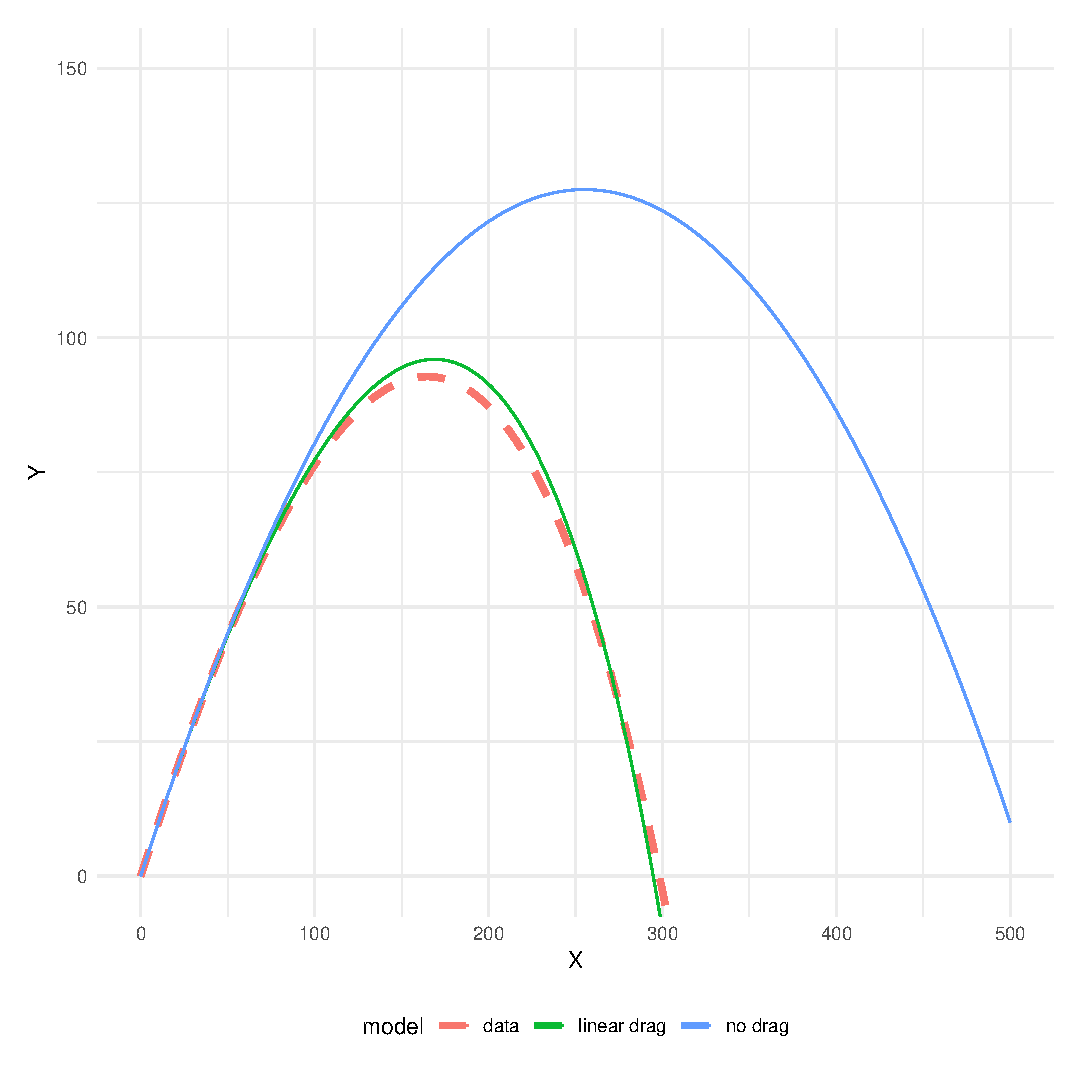
\includegraphics[width=0.85\textwidth]{./images/projectile_traj}

  \caption{Projectile trajectories using different drag models. Clearly, the `no
    drag' option does not match the observed data; the model is in error.
    However, even after tuning the drag coefficient, the `linear drag' model
    still does not match the data; the \emph{functional form} of the drag model
    is in error, leading to model form uncertainty.}
  \label{fig:projectile-traj}
\end{figure}

As engineers and scientists with years of training in physics, it is easy --
perhaps pedantic -- for us to clearly articulate the phenomena lost in dragless
projectile motion. However, the same sort of \emph{model error} is present in
more complicated problems -- errors which we may not even know exist. To help in
identifying cases where model form uncertainty may be present, we introduce a
few interrelated concepts that characterize these errors.

\textbf{Missing physics} is a simple enough concept, though unknown unknowns are
always difficult to treat. The Tacoma Narrows Bridge is the quintessential
example of how things can go horribly wrong when physical phenomena are simply
not accounted. The 1940's bridge design was carried out under static wind load
conditions, as dynamic wind loading was seen as secondary to the huge weight of
the stationary structure.\cite{scott2003} The bridge's eventual collapse was due
to dynamic phenomena, though the precise mechanism is still
debated.\cite{billah1991resonance}

This sort of error can occur when one moves into an unfamiliar domain; either in
terms of fields of study, or when moving to different physical \emph{scales}.

\textbf{Scale} is an ubiquitous concept in physics, and often forms the
boundaries between disciplines. While many physical phenomena change
continuously across changes in length-, time-, mass-, and other-scales,
qualitative changes occur as well. Clearly, if qualitative changes are not
accounted in physical models, then there will be some form of discrepancy.
However, the surprises in moving to a different field can be humbling.

As a mechanical engineer with a background in fluids and aircraft, I often
regarded the momentum imparted by photons as an academic curiosity, perhaps of
interest to those designing solar sails. I was personally astounded to learn
from graduate student colleagues that satellite designers have to account for
\emph{solar radiation pressure} in their designs! When the ambient force-scales
are in micro-Newtons, such `small' effects become quite
relevant.\footnote{Designers of the Internation Space Station had to account for
  the difference in Earth's graviational attraction across the station, as the
  structure is large enough that a non-negligible \emph{graviational moment} is
  applied!}

Neglecting radiation pressure on aircraft is possible due to \emph{scale
  separation} -- the pressure contributions due to photons are so small compared
to fluid pressure that the phenomena can be neglected without much consequence.
`New' phenomena can become relevant when the scales of interest change
dramatically, but more subtle effects can occur due to scale
\emph{interactions}.

\textbf{Interaction} is the generic term we give to phenomena, usually
considered separately, that work together to produce some effect. Interactions
are most obvious when domains cross, such as when fluids and structures interact
to produce aeroelastic flutter. Such effects can also occur within a single
domain; perhaps the most famout example is the so-called butterfly effect, where
in nonlinear dynamical systems, small-scale perturbations can lead to large
(infinite) divergences in finite time. Here, the surprising interaction is
between scales, usually thought to be separated in behavior -- this is a key
feature of turbulence.\cite{pope2001turbulent}

How can we handle model form uncertainty? Higdon et
al.\cite{higdon2004calibration-prediction} suggest a means to fuse information
available from physical and simulation data, and build an approximation to the
discrepancy between the two sets. Their approach is to construct a discrepancy
function $\delta(\vx)$\footnote{specifically, they use \emph{gaussian process
    regression} to construct this function} such that

\begin{equation}
  y_i = f(\vx_i) + \delta(\vx_i) + \epsilon_i,
\end{equation}

\noindent where $f$ is the simulation output, $\epsilon_i$ is experimental
error, $\delta$ represents model form uncertainty, and the $y_i$ are physical
data, collected at nominal conditions $\vx_i$. They admit that extrapolating
beyond the collected data $\{y_i,\vx_i\}$ can be challenging, and note that such
a procedure is most defensible when used to study conditions within the confines
of available data. One can use this discrepancy to improve predictions, or as a
means to inform further modifications to a model.\cite{joseph2015engineering}

%% --------------------------------------------------
\section{Sensitivity Analysis} \label{sec:sa}
%% --------------------------------------------------
Above, we posed the question ``Is the uncertainty in $Y$ significant?'' A full
answer to this question requires choosing a context and computing the
uncertainty in $Y$. \textbf{Sensitivity analysis} asks a slightly different
question: ``How do uncertainties in $\mX$ affect those in $Y$?'' First studying
the sensitivity of a model $f(\cdot)$ can identify the inputs which are most
important to $Y$, which has multiple benefits.

For instance, one might be interested in reducing the uncertainty in $Y$, and
would like to determine a subset of $\mX$ for further study, in order to reduce
input uncertainty for a subset of variables. Sensitivity analysis can also allow
one to determine if particular inputs are \emph{unimportant}, with regard to the
output uncertainty. This enables one to fix these unimportant inputs to nominal
values, making uncertainty propagation cheaper, possibly rendering an
intractable computational problem feasible.

A different perspective on the same use is to determine what physical data is
most worth gathering. Clearly, if the output of interest $y$ is insensitive to a
particular input $x_i$, then gathering more data on this predictor is not a
useful exercise. Sensitivity analysis on a model can help to inform follow-up
experiments, which can be useful to support the allocation of scientific and
engineering resources. However, it is important to note that all sensitivity
being studied is that of the \emph{model}, and not of \emph{physics} -- if the
model is not an accurate description of reality, the resulting analysis may be
misleading!

There are at least two broad families of sensitivity analysis: local and global.
Figure \ref{fig:local-vs-global} provides a cartoon example, intended to
illustrate the difference and need for these two separate, broad mentalities.

\begin{figure}[!ht]
  \centering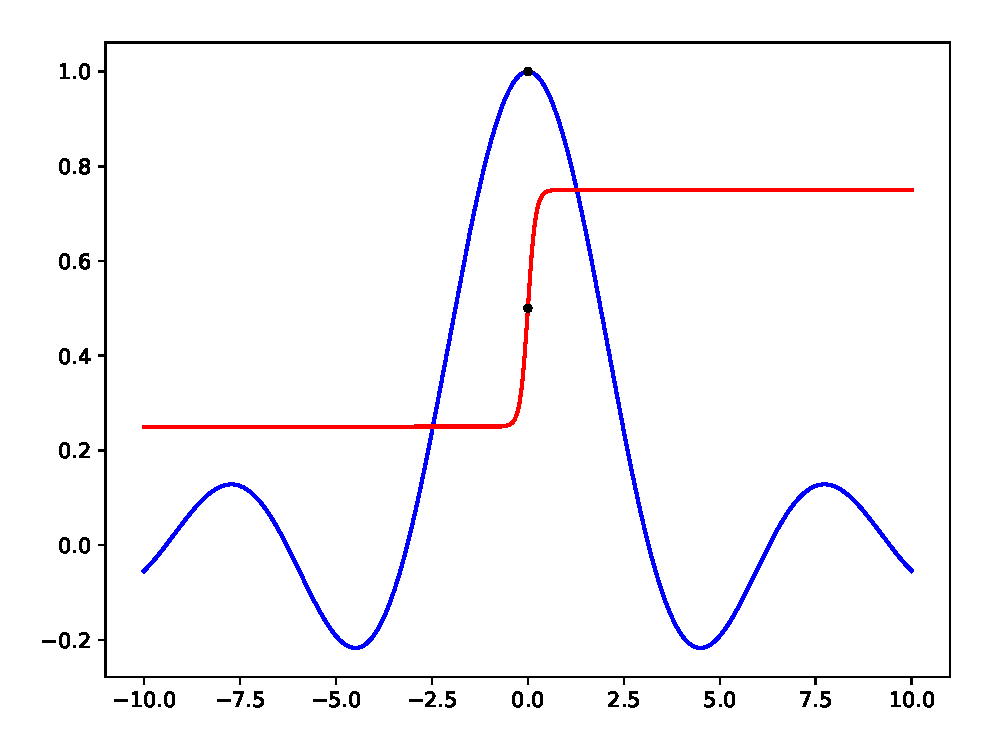
\includegraphics[width=0.75\textwidth]{./images/local_vs_global}
  \caption{Cartoon functions to depict differences between local and global
    sensitivity. The vertical axis corresponds to the output qoi, while the
    horizontal corresponds to an input quantity. The black dot is the point of
    interest for local sensitivity. The blue curve has a great deal of global
    sensitivity, but zero local sensitivity. The red curve has comparatively
    little global sensitivity, but a large local sensitivity. Which metric is
    important depends on the objective of the study.}
  \label{fig:local-vs-global}
\end{figure}

\textbf{Local sensitivity analysis} usually refers to computing derivatives of
an output quantity $y$ with respect to the inputs $\vx$.\footnote{Sometimes
  `sensitivity' is used interchangeably with `derivative'.} A local analysis is
appropriate when one is interested in the behavior at and around `special'
points in the domain $\cD$. For example, we might be interested in the stability
of an optimal value for a constrained optimization problem -- a local
sensitivity analysis would aid in this study.\footnote{The Karush-Kuhn-Tucker
  conditions formalize some -- but not all -- aspects of this sort of
  sensitivity analysis.\cite{boyd2004convex}}

\textbf{Global sensitivity analysis} usually refers to attributing
\emph{variability} in the output $y$ to the different inputs $\vx$. Often,
variability is quantified in terms of variance.\footnote{though alternatives
  exist; for instance one may seek to attribute portions of skewness, kurtosis,
  or other moments to different inputs.\cite{owen2014higher}} For example, we
might be interested in determining which single input $X_i$ contributes the most
variance to the output $Y$, in order to better characterize the distribution of
$X_i$ and ultimate reduce uncertainty in the output.

As implied by the names, the two mentalities seek different pieces of
information. Depending on the context, one or the other may be the `right'
perspective to adopt. Figure \ref{fig:local-vs-global} provides a simple cartoon
illustration of two cases where local and global sensitivities will be in
disagreement.

\subsection{Local Sensitivity Analysis}
%% -------------------------
\textcolor{red}{TODO} Motivation

Local sensitivity analysis can be accomplished in a rather straightforward
fashion via a \textbf{finite difference}. For a first-order approximation, one
simply chooses a base point $\vx$ and considers a finite step-size $\Delta x$
approximation to the (partial) derivative

\begin{equation}
  \frac{\partial f}{\partial x_i} \approx \frac{f(x_1,\dots,x_i+\Delta
    x,\dots,x_d) - f(\vx)}{\Delta x}.
\end{equation}

However, there are some complications with this approach. The first challenge is
choosing a sensible $\Delta x$. A common heuristic is to use the square root of
floating point machine precision. Recent work has studied the selection of
$\Delta x$ based on measuring the \emph{empirical noise} of a function; that is,
tailoring the step-size based on the observered variability in a computed qoi
arising from a computational procedure.\cite{more2012}\footnote{I have found the
  work of Mor{\'e} and Wild to be very helpful in my own work, and often use my
  own \href{https://github.com/zdelrosario/pyutil}{python implementation} of
  their algorithm for approximating an appropriate step size.}

Second, this computational procedure requires additional evaluations, with a
cost that grows linearly with dimensionality $d$. If we require $N$ evaluations
of the gradient for a desired procedure (e.g. building a map of the gradient or
performing quadrature), then our total cost will be $O(Nd)$. Despite the low
growth rate, when studying costly simulations, the additional expense can
quickly render finite differences intractable. The adjoint method is a possible
solution to this issue.

The adjoint is clever method for cheaply computing the sensitivity of a scalar
qoi. This is particularly useful if evaluating our qoi requires solving some
parameterized governing equation $F(\vy,\vx)$ for a state variable (e.g. flow
field) on which our qoi depends $f(\vy,\vx)$. Practically, it allows us to
compute the total derivative of our qoi $\frac{df}{d\vx}$ at the expense of one
additional solution comparable to $F(\vy,\vx)$.\footnote{While the finite
  difference method grew linearly in the number of variables, the adjoint method
  grows linearly in the number of \emph{output quantities} we wish to study.
  There is a tradeoff in this business; if we have more outputs than inputs,
  then finite differences may be the best choice.} Steven Johnson
\cite{johnson2012} has some very nice introductory notes on the topic, which I
follow for the next example. He also points to a paper by Cao et
al.\cite{cao2003adjoint} which gives a more general treatment of the adjoint.

The spirit of the adjoint method is well-illustrated by a simple linear system.
Suppose we have a governing equation for the state
$A_{jk}(\vx)y_k=b_j(\vx)$ \footnote{We'll use
  \href{https://en.wikipedia.org/wiki/Einstein_notation}{Einstein notation} here
  to help make this easier to follow.}, where our equation is parameterized by
$\vx$. Our qoi is some known function of the state and our parameters
$f(\vy,\vx)$. By chain rule, the sensitivity is

\begin{equation}\label{eq:linear-sens}
  \frac{df}{dx_i} = \frac{\partial f}{\partial x_i} %
                  + \frac{\partial f}{\partial y_j}\frac{\partial y_j}{\partial x_i}.
\end{equation}

\noindent Since $f$ is known, the partials $\frac{\partial f}{\partial x_i}$ and
$\frac{\partial f}{\partial y_j}$ are easy to evaluate.\footnote{Here, we use
  $\partial$ to denote a `direct' derivative. For example, if
  $f(\vx,\vy)=\sum_{i=j}^my_j$, then $\frac{\partial f}{\partial x_i}=0$ and
  $\frac{\partial f}{\partial y_j}=1$.} However, the quantity $\frac{\partial
  y_j}{\partial x_i}$ is more challenging. Using the matrix inverse, we have
$y_j=A_{jk}^{-1}b_k$. Taking the partial, we have \footnote{Here, we use the
  identity $\frac{\partial \mA^{-1}}{\partial s} =-\nobreak
  \mA^{-1}\frac{\partial \mA}{\partial s}\mA^{-1}$. One can derive this by
  re-arranging $\frac{\partial(\mA^{-1}\mA)}{\partial s}$.}

\begin{equation} \begin{aligned}
  \frac{\partial y_j}{\partial x_i} &= \frac{\partial A^{-1}_{jk}}{\partial x_i}b_k + A^{-1}_{jk}\frac{\partial b_k}{\partial x_i}, \\
  &= A^{-1}_{jk}\left(-\frac{\partial A_{kl}}{\partial x_i}A^{-1}_{lp}b_p+\frac{\partial b_k}{\partial x_i}\right), \\
  &= A^{-1}_{jk}\left(-\frac{\partial A_{kl}}{\partial x_i}x_l+\frac{\partial b_k}{\partial x_i}\right).
\end{aligned} \end{equation}

\marginnote{Using Einstein notation makes it clear in \eqref{eq:linear-sens2}
  that the quantity $\frac{\partial A_{kl}}{\partial x_i}$ is a rank 3 tensor,
  as there are three indices.}

\noindent Substituting into \eqref{eq:linear-sens} yields

\begin{equation}\label{eq:linear-sens2}
  \frac{df}{dx_i} = \frac{\partial f}{\partial x_i} + \frac{\partial f}{\partial y_j}A^{-1}_{jk}%
  \left(-\frac{\partial A_{kl}}{\partial x_i}y_l + \frac{\partial b_k}{\partial x_i}\right).
\end{equation}

One could evaluate \eqref{eq:linear-sens2} by carrying out the matrix
multiplication (which would be expensive), or by carrying out the product
$\frac{\partial f}{\partial y_j}A^{-1}_{jk}\equiv\nobreak\lambda_k$. This
quantity is the solution of the \emph{adjoint equation}

\begin{equation}\label{eq:linear-adjoint}
  \lambda_k A_{kj} = \frac{\partial f}{\partial y_j}.
\end{equation}

In summary, to compute the sensitivity via the adjoint method, we need (1) the
solution to the governing equation $\vy$ at our chosen parameter values, (2) the
partial derivatives to known functions $\frac{\partial f}{\partial x_i},
\frac{\partial f}{\partial y_j}, \frac{\partial A_{kl}}{\partial x_i},
\frac{\partial b_k}{\partial x_i}$, and (3) the solution to the adjoint equation
$\lambda_k$. We then evaluate the total derivative via

\begin{equation}
  \frac{df}{dx_i} = \frac{\partial f}{\partial x_i} +
    \lambda_k A^{-1}_{jk}\left(-\frac{\partial A_{kl}}{\partial x_i}y_l +
    \frac{\partial b_k}{\partial x_i}\right).
\end{equation}

\textcolor{red}{TODO} Example

\subsection{Global Sensitivity Analysis}
%% -------------------------
Why perform global sensitivity analysis? One reason is to perform
\emph{dimension reduction}; that is, principled reduction of the dimensionality
of a system. Figure \ref{fig:curse} depicts the \emph{curse of dimensionality},
which states (roughly) that the computational expense of a procedure tends to
grow \emph{exponentially} with the dimension of the problem. The most direct way
to address this issue is to reduce dimensionality -- to reduce the number of
input parameters we need to consider.

Suppose we perform a sensitivity analysis and find that our qoi $f(\vx)$ is
relatively unaffected by its input $x_1$. We could set $x_1=c$ to a constant
nominal value, and continue with $f(c,x_2,\dots,x_d)$, which has dimension
$d-1$. This would reduce the expense involved with studying our qoi, and since
the reduction is \emph{exponential} this could potentially enable studies
previous intractable. Global sensitivity analysis provides principled tools to
perform dimension reduction.

\begin{figure}[!ht]
  \centering
  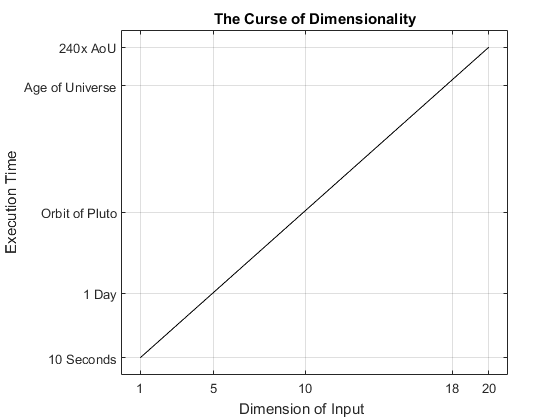
\includegraphics[width=0.75\textwidth]{./images/curse_of_dimensionality}
  \caption{Cartoon depicting computational expense under the Curse of Dimensionality.
  The most direct way to address this curse is to reduce the effective dimension
  of our problem. One way to reduce dimensionality is to identify parameters
  which are unimportant, and freeze them to nominal values. Global sensitivity
  analysis allows us to determine such unimportant factors.}
  \label{fig:curse}
\end{figure}

We'll briefly mention two methods for global sensitivity analysis: Morris
Screening, which seeks to identify unimportant parameters in an economical
fashion, and Active Subspaces, which identify important directions in parameter
space. Finally, we'll study Sobol' Indices in detail, which attribute
variability in an output to subsets of the inputs.

\textbf{Morris screening} is closely related to the local sensitivities, and can
be thought of as studying the mean and variance of the derivative. Ralph Smith's
textbook \cite{smith2013uncertainty} goes through this procedure in gory detail;
we'll go through a very brief introduction here. Morris screening considers
statistics of the \emph{elementary effects}, defined by

\begin{equation}\label{eq:elem-effect}
  d_{i}(\vx_j) = \frac{f(\vx_j+\Delta \ve_i) - f(\vx_j)}{\Delta},
\end{equation}

\noindent where $\ve_i$ is the i-th standard basis vector,\footnote{The vector
  with all zeros, except for a one in the i-th entry} and $\Delta$ is a large
stepsize. Note that \eqref{eq:elem-effect} is simply a first-order approximation
of the derivative; however, since $\Delta$ is relatively large, this is a coarse
approximation to the derivative. These elementary effects are used to construct
global sensitivity measures

\begin{equation}\begin{aligned}
  \mu_i^* &= \frac{1}{r}\sum_{j=1}^r |d_{i}(\vx_j)|, \\
  \sigma_i^2 &= \frac{1}{r-1}\sum_{j=1}^r(d_{i}(\vx_j)-\mu_i)^2, \mu_i=\frac{1}{r}\sum_{j=1}^rd_{i}(\vx_).
\end{aligned}\end{equation}

Note that considering elementary effects misses interactions, for the reasons
discussed above. Generalizations of this technique consider higher-order
derivatives, which probe interactions. This procedure is called \emph{screening}
because it allows us to determine whether individual parameters are unimportant,
but does not quantify relative variable importance. To determine relative
importance, we can turn to Sobol indices. However, Morris screening is a
relatively cheap procedure, and thus is a good tool to be aware of.

The \textbf{active subspace} is a more recent dimension reduction technique, and
is somewhat different in spirit from other global sensitivity analysis
procedures.\cite{constantine2015} Consider the function

\begin{equation}\label{eq:as-ex}
  f(\vx) = \f12(0.3x_1+0.7x_2)^2.
\end{equation}

\noindent For this qoi, both its parameters are important. However, the function
clearly varies only along the direction $(0.3,0.7)^T$, and not at all along the
direction $(0.7,-0.3)^T$. Rather than picking and freezing individual
parameters, the active subspace considers \emph{linear combinations} of the
inputs which are important. These correspond to directions in parameter space.
Figure \ref{fig:as-ex} depicts the active subspace for \eqref{eq:as-ex}.

\begin{figure}[!ht]
  \centering
  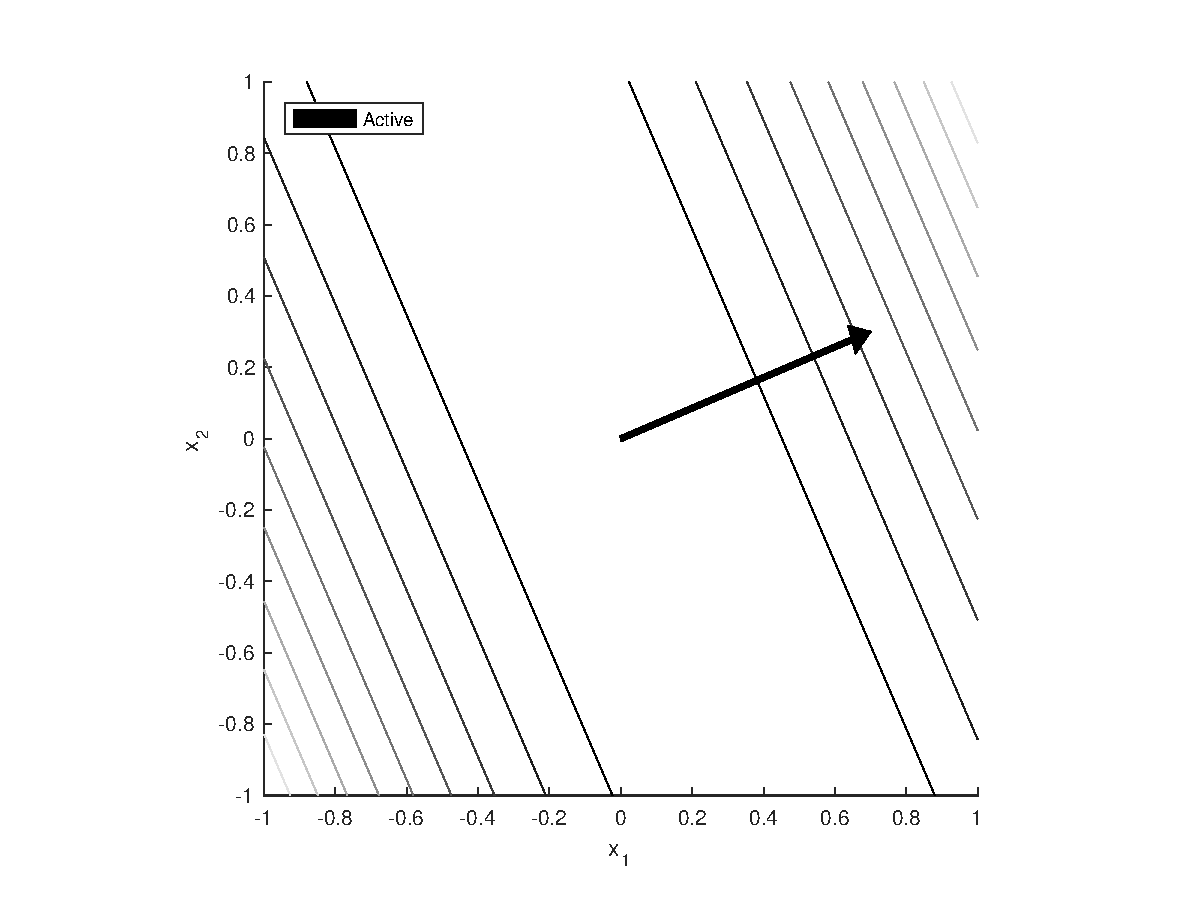
\includegraphics[width=0.75\textwidth]{./images/contour_plot}
  \caption{Isolines and active direction for \eqref{eq:as-ex}}
  \label{fig:as-ex}
\end{figure}

The active subspace is computed by studying the outer product of the gradient;
taking an expectation with respect to the density for $\vx$, we define

\begin{equation}\label{eq:as-c}
  \mC = \E[\nabla_{\vx}f\nabla_{\vx}f^T].
\end{equation}

\noindent Note that $\mC$ is symmetric semi-positive definite, thus it admits an
eigenvalue decomposition $\mC=\mW\m\Lambda\mW^T$. A basis for the active
subspace is identified by separating the magnitude-ordered eigenvalues
$\m\Lambda=\text{Diag}([\m\Lambda_a,\m\Lambda_i])$ and their associated
eigenvectors $\mW=[\mW_a,\mW_i]$. This split is often chosen based on the
relative magnitude of the eigenvalues.

In contrast with Morris screening, we may use the eigenvalues $\lambda_i$ to
rank the associated directions $\vw_i$. The $\lambda_i$ are related to the
mean-squared directional derivative associated with the appropriate eigenvector.
Thus, ranking the directions can only be done in an average sense; the
eigenvalues may hide extreme local behavior. Furthermore, the active subspace
requires gradient information; this is fine if we access to this information,
say through an adjoint solver. If gradients are unavailable, we would need to
turn to other approaches, such as finite differences or surrogate modeling,
which increases the expense.

Exploiting the active subspace involves a number of challenges, and is both
application dependent and an active area of research. To illustrate some of
these challenges, suppose we define the \emph{active} and \emph{inactive
  variables} based on the decomposition above

\begin{equation}\begin{aligned}
  \vx_a &= \mW^T_a\vx, \\
  \vx_i &= \mW^T_i\vx.
\end{aligned}\end{equation}

\noindent We would like to re-parameterize our qoi in terms of the $\vx_a$ to
reduce dimensionality. However, the naive statement $f(\vx)=f(\mW_a\vx_a)$ is
false! Furthermore, we must determine the domain of $\vx_a$; this is a
projection of the original domain $\Omega$ on the subspace $\cR(\mW_a)$, which
is in general quite complicated.

Both Morris screening and the active subspace consider some average of the
gradient. In contrast, \textbf{Sobol' indices} are based on \emph{variance}.
Sobol' indices may be used to attribute variance of the qoi to subsets of the
input parameters. It is a useful, well-studied, and commonly-used technique for
global sensitivity analysis, so we will spend some time discussing it.

Sobol' indices require a random variable interpretation of our quantity of
interest, so we'll introduce some notation used throughout the section. Let
$\mX\sim\rho$ be our random input parameters, distributed according to a joint
density $\rho$ over our parameter space $\Omega$.\footnote{Sobol indices also
  have some properties that rely on \emph{independence} of the input parameters.
  We will return to this point later.} Then our output qoi is also a random
variable $Y=f(\mX)$. We denote by $\E[Y] = \int f(\vx)\rho(\vx)d\vx$ the
expectation, and by $\V[Y]=\E[(Y-\E[Y])^2]$ the variance. Note that the
following useful identity involving the variance holds

\begin{equation}
  \V[Y] = \E[Y^2] - \E[Y]^2.
\end{equation}

We denote conditioning by a vertical bar; this corresponds to holding particular
random inputs fixed in value, and leaving them out of the integral for a
particular expectation. For example, if $Y=f(X_1,X_2,X_3)$, then

\begin{equation}
  \E_{X_2,X_3}[Y|X_1=x_1] = \int f(x_1,x_2,x_3)\rho(x_1,x_2,x_3)dx_2dx_2,
\end{equation}

\noindent where we use subscripts to make explicit the integration variables.
Note that $\E_{X_2,X_3}[Y|X_1]$ is still a random variable\footnote{when it
  lacks the equality $X_1=x_1$}, due to the variability arising from $X_1$. We
will use conditional variance to decompose the total variance $\V[Y]$ according
to different input contributions. This will involve expressions of the sort
$\E_{X_2,X_2}[\V_{X_1}[Y|X_1]]$.\footnote{which is no longer a random variable,
  as we have integrated out all of the parameters}

In what follows, we will drop the variable subscripts, as they tend to render
expressions indecipherable. The same information is implied by the conditioning;
the expression $\V[Y|X_1]$ carries out the integration keeping $X_1$ fixed,
which is then integrated out in the expression $\E[\V[Y|X_1]]$.

Rather than trudge through a formal derivation of Sobol' indices, we will step
through a simple treatment of Sobol' indices, in order to build intuition. For a
more formal treatment, see Owen (2013).\cite{owen2013variance}

The Sobol indices are based on a decomposition of the variance of our output
qoi.\footnote{This necessitates a random variable interpretation of both our
  inputs and outputs. In the absence of `truly' random inputs, one can assign
  uniform distributions to the uncertain parameters.} In the next section, we'll
look at a formal treatment using the functional analysis of variance. Before
that, we'll go through a more simple treatment of the same problem, in order to
build intuition.\footnote{The primer by Saltelli et
  al.\cite{saltelli2004sensitivity} is a good, quick read on sensitivity
  analysis. I follow that text for this subsection.}

First, we will introduce some notation to help keep track of variable subsets.
Let $\vu$ be an \emph{index set}; that is $\vu\subseteq\{1,\dots,d\}$. We will
use $\vu$ to denote subsets of the input variables; in the example above, we
used $\vu=\{2,3\}$ to give us $\mX_{\vu}=\{X_2,X_3\}$. Let $-\vu$ be the set
complementary to $\vu$ with respect to $\{1,\dots,d\}$; in the example above
$-\vu=\{1\}$.

Next, we will prove a simple identity, which will allow us to attribute the
variance $\V[Y]$ to different inputs. Note that for any index set $\vu$, we have

\begin{equation}\begin{aligned}\label{eq:var-decomp}
  \E[\V[Y|\mX_{\vu}]] + \V[\E[Y|\mX_{\vu}]] &= %
  \E[\E[Y^2|\mX_{\vu}] - \cancel{ \E[Y|\mX_{\vu}]^2 }] \\
  &+ \cancel{\E[\E[Y|\mX_{\vu}]^2]} - \E[\E[Y|\mX_{\vu}]]^2, \\
  &= \E[Y^2] - \E[Y]^2, \\
  &= \V[Y^2].
\end{aligned}\end{equation}

\noindent \Cref{eq:var-decomp} allows us to decompose the variance into two
terms \emph{that we can interpret}. First, note that the expression
$\V[\E[Y|X_{\vu}]]$ first averages out all the variables $\mX_{-\vu}$, then
computes the variance due only to $\mX_{\vu}$. We may use this expression with a
singleton index set $\vu=\{i\}$ to define the \textbf{first-order sensitivity
  index}

\begin{equation}\label{eq:sobol-first}
  \underline{\tau}_{\{i\}}^2 = \frac{\V[\E[Y|X_i]]}{\V[Y]}.
\end{equation}

\noindent \Cref{eq:sobol-first} is bounded between $[0,1]$, and enables us to
rank variables according to their importance. Practically
$\underline{\tau}_{\{i\}}^2$ tells us how much variance reduction we could
expect if we were able to exactly freeze $\mX_i$. We could use this information
to inform which variables we should better characterize, in order to reduce
variability.

Note that we should \emph{not} use $\underline{\tau}_{\{i\}}^2$ to perform
dimension reduction; the first-order index does not account for interactions
with other variables, so we may miss some important cross terms. Instead, we may
consider the \textbf{total-order sensitivity index}

\begin{equation}\label{eq:sobol-total}
  \overline{\tau}_{\{i\}}^2 = \frac{\E[\V[Y|X_{-\{i\}}]]}{\V[Y]} = %
  1 - \frac{\V[\E[Y|X_{-\{i\}}]]}{\V[Y]}.
\end{equation}

\noindent \Cref{eq:sobol-total} is also bounded between $[0,1]$, and accounts
for interactions between $X_i$ and all other variables. We may interpret
\eqref{eq:sobol-total} in at least two ways: As the variability in $Y$ due to
$X_i$, averaged over all other inputs (middle expression), or as the complement
of the variability arising from all the variables excluding $X_i$ (right
expression). If $\overline{\tau}_{\{i\}}^2$ is zero or small, we can be
confident that $X_i$ contributes little to the variablility in $Y$, neither
through first-order nor interaction effects.

In summary: The notation for the sensitivity indices is suggestive of their use.
The first-order index $\underline{\tau}_{\{i\}}^2$ can be thought of as a
\emph{lower} bound; if it is large, then we can be confident that $X_i$ is
\emph{important}. In contrast the total-order index $\overline{\tau}_{\{i\}}^2$
is an \emph{upper} bound; if it is small, then we can be confident that $X_i$ is
\emph{unimportant}.

\textcolor{red}{TODO} Example

\end{document}
